% Options for packages loaded elsewhere
\PassOptionsToPackage{unicode}{hyperref}
\PassOptionsToPackage{hyphens}{url}
%
\documentclass[
  letterpaper,
  DIV=11,
  numbers=noendperiod]{scrartcl}

\usepackage{amsmath,amssymb}
\usepackage{iftex}
\ifPDFTeX
  \usepackage[T1]{fontenc}
  \usepackage[utf8]{inputenc}
  \usepackage{textcomp} % provide euro and other symbols
\else % if luatex or xetex
  \usepackage{unicode-math}
  \defaultfontfeatures{Scale=MatchLowercase}
  \defaultfontfeatures[\rmfamily]{Ligatures=TeX,Scale=1}
\fi
\usepackage{lmodern}
\ifPDFTeX\else  
    % xetex/luatex font selection
\fi
% Use upquote if available, for straight quotes in verbatim environments
\IfFileExists{upquote.sty}{\usepackage{upquote}}{}
\IfFileExists{microtype.sty}{% use microtype if available
  \usepackage[]{microtype}
  \UseMicrotypeSet[protrusion]{basicmath} % disable protrusion for tt fonts
}{}
\makeatletter
\@ifundefined{KOMAClassName}{% if non-KOMA class
  \IfFileExists{parskip.sty}{%
    \usepackage{parskip}
  }{% else
    \setlength{\parindent}{0pt}
    \setlength{\parskip}{6pt plus 2pt minus 1pt}}
}{% if KOMA class
  \KOMAoptions{parskip=half}}
\makeatother
\usepackage{xcolor}
\setlength{\emergencystretch}{3em} % prevent overfull lines
\setcounter{secnumdepth}{4}
% Make \paragraph and \subparagraph free-standing
\makeatletter
\ifx\paragraph\undefined\else
  \let\oldparagraph\paragraph
  \renewcommand{\paragraph}{
    \@ifstar
      \xxxParagraphStar
      \xxxParagraphNoStar
  }
  \newcommand{\xxxParagraphStar}[1]{\oldparagraph*{#1}\mbox{}}
  \newcommand{\xxxParagraphNoStar}[1]{\oldparagraph{#1}\mbox{}}
\fi
\ifx\subparagraph\undefined\else
  \let\oldsubparagraph\subparagraph
  \renewcommand{\subparagraph}{
    \@ifstar
      \xxxSubParagraphStar
      \xxxSubParagraphNoStar
  }
  \newcommand{\xxxSubParagraphStar}[1]{\oldsubparagraph*{#1}\mbox{}}
  \newcommand{\xxxSubParagraphNoStar}[1]{\oldsubparagraph{#1}\mbox{}}
\fi
\makeatother

\usepackage{color}
\usepackage{fancyvrb}
\newcommand{\VerbBar}{|}
\newcommand{\VERB}{\Verb[commandchars=\\\{\}]}
\DefineVerbatimEnvironment{Highlighting}{Verbatim}{commandchars=\\\{\}}
% Add ',fontsize=\small' for more characters per line
\usepackage{framed}
\definecolor{shadecolor}{RGB}{241,243,245}
\newenvironment{Shaded}{\begin{snugshade}}{\end{snugshade}}
\newcommand{\AlertTok}[1]{\textcolor[rgb]{0.68,0.00,0.00}{#1}}
\newcommand{\AnnotationTok}[1]{\textcolor[rgb]{0.37,0.37,0.37}{#1}}
\newcommand{\AttributeTok}[1]{\textcolor[rgb]{0.40,0.45,0.13}{#1}}
\newcommand{\BaseNTok}[1]{\textcolor[rgb]{0.68,0.00,0.00}{#1}}
\newcommand{\BuiltInTok}[1]{\textcolor[rgb]{0.00,0.23,0.31}{#1}}
\newcommand{\CharTok}[1]{\textcolor[rgb]{0.13,0.47,0.30}{#1}}
\newcommand{\CommentTok}[1]{\textcolor[rgb]{0.37,0.37,0.37}{#1}}
\newcommand{\CommentVarTok}[1]{\textcolor[rgb]{0.37,0.37,0.37}{\textit{#1}}}
\newcommand{\ConstantTok}[1]{\textcolor[rgb]{0.56,0.35,0.01}{#1}}
\newcommand{\ControlFlowTok}[1]{\textcolor[rgb]{0.00,0.23,0.31}{\textbf{#1}}}
\newcommand{\DataTypeTok}[1]{\textcolor[rgb]{0.68,0.00,0.00}{#1}}
\newcommand{\DecValTok}[1]{\textcolor[rgb]{0.68,0.00,0.00}{#1}}
\newcommand{\DocumentationTok}[1]{\textcolor[rgb]{0.37,0.37,0.37}{\textit{#1}}}
\newcommand{\ErrorTok}[1]{\textcolor[rgb]{0.68,0.00,0.00}{#1}}
\newcommand{\ExtensionTok}[1]{\textcolor[rgb]{0.00,0.23,0.31}{#1}}
\newcommand{\FloatTok}[1]{\textcolor[rgb]{0.68,0.00,0.00}{#1}}
\newcommand{\FunctionTok}[1]{\textcolor[rgb]{0.28,0.35,0.67}{#1}}
\newcommand{\ImportTok}[1]{\textcolor[rgb]{0.00,0.46,0.62}{#1}}
\newcommand{\InformationTok}[1]{\textcolor[rgb]{0.37,0.37,0.37}{#1}}
\newcommand{\KeywordTok}[1]{\textcolor[rgb]{0.00,0.23,0.31}{\textbf{#1}}}
\newcommand{\NormalTok}[1]{\textcolor[rgb]{0.00,0.23,0.31}{#1}}
\newcommand{\OperatorTok}[1]{\textcolor[rgb]{0.37,0.37,0.37}{#1}}
\newcommand{\OtherTok}[1]{\textcolor[rgb]{0.00,0.23,0.31}{#1}}
\newcommand{\PreprocessorTok}[1]{\textcolor[rgb]{0.68,0.00,0.00}{#1}}
\newcommand{\RegionMarkerTok}[1]{\textcolor[rgb]{0.00,0.23,0.31}{#1}}
\newcommand{\SpecialCharTok}[1]{\textcolor[rgb]{0.37,0.37,0.37}{#1}}
\newcommand{\SpecialStringTok}[1]{\textcolor[rgb]{0.13,0.47,0.30}{#1}}
\newcommand{\StringTok}[1]{\textcolor[rgb]{0.13,0.47,0.30}{#1}}
\newcommand{\VariableTok}[1]{\textcolor[rgb]{0.07,0.07,0.07}{#1}}
\newcommand{\VerbatimStringTok}[1]{\textcolor[rgb]{0.13,0.47,0.30}{#1}}
\newcommand{\WarningTok}[1]{\textcolor[rgb]{0.37,0.37,0.37}{\textit{#1}}}

\providecommand{\tightlist}{%
  \setlength{\itemsep}{0pt}\setlength{\parskip}{0pt}}\usepackage{longtable,booktabs,array}
\usepackage{calc} % for calculating minipage widths
% Correct order of tables after \paragraph or \subparagraph
\usepackage{etoolbox}
\makeatletter
\patchcmd\longtable{\par}{\if@noskipsec\mbox{}\fi\par}{}{}
\makeatother
% Allow footnotes in longtable head/foot
\IfFileExists{footnotehyper.sty}{\usepackage{footnotehyper}}{\usepackage{footnote}}
\makesavenoteenv{longtable}
\usepackage{graphicx}
\makeatletter
\newsavebox\pandoc@box
\newcommand*\pandocbounded[1]{% scales image to fit in text height/width
  \sbox\pandoc@box{#1}%
  \Gscale@div\@tempa{\textheight}{\dimexpr\ht\pandoc@box+\dp\pandoc@box\relax}%
  \Gscale@div\@tempb{\linewidth}{\wd\pandoc@box}%
  \ifdim\@tempb\p@<\@tempa\p@\let\@tempa\@tempb\fi% select the smaller of both
  \ifdim\@tempa\p@<\p@\scalebox{\@tempa}{\usebox\pandoc@box}%
  \else\usebox{\pandoc@box}%
  \fi%
}
% Set default figure placement to htbp
\def\fps@figure{htbp}
\makeatother
% definitions for citeproc citations
\NewDocumentCommand\citeproctext{}{}
\NewDocumentCommand\citeproc{mm}{%
  \begingroup\def\citeproctext{#2}\cite{#1}\endgroup}
\makeatletter
 % allow citations to break across lines
 \let\@cite@ofmt\@firstofone
 % avoid brackets around text for \cite:
 \def\@biblabel#1{}
 \def\@cite#1#2{{#1\if@tempswa , #2\fi}}
\makeatother
\newlength{\cslhangindent}
\setlength{\cslhangindent}{1.5em}
\newlength{\csllabelwidth}
\setlength{\csllabelwidth}{3em}
\newenvironment{CSLReferences}[2] % #1 hanging-indent, #2 entry-spacing
 {\begin{list}{}{%
  \setlength{\itemindent}{0pt}
  \setlength{\leftmargin}{0pt}
  \setlength{\parsep}{0pt}
  % turn on hanging indent if param 1 is 1
  \ifodd #1
   \setlength{\leftmargin}{\cslhangindent}
   \setlength{\itemindent}{-1\cslhangindent}
  \fi
  % set entry spacing
  \setlength{\itemsep}{#2\baselineskip}}}
 {\end{list}}
\usepackage{calc}
\newcommand{\CSLBlock}[1]{\hfill\break\parbox[t]{\linewidth}{\strut\ignorespaces#1\strut}}
\newcommand{\CSLLeftMargin}[1]{\parbox[t]{\csllabelwidth}{\strut#1\strut}}
\newcommand{\CSLRightInline}[1]{\parbox[t]{\linewidth - \csllabelwidth}{\strut#1\strut}}
\newcommand{\CSLIndent}[1]{\hspace{\cslhangindent}#1}

\usepackage{lscape}
\newcommand{\blandscape}{\begin{landscape}}
\newcommand{\elandscape}{\end{landscape}}
\KOMAoption{captions}{tableheading}
\makeatletter
\@ifpackageloaded{tcolorbox}{}{\usepackage[skins,breakable]{tcolorbox}}
\@ifpackageloaded{fontawesome5}{}{\usepackage{fontawesome5}}
\definecolor{quarto-callout-color}{HTML}{909090}
\definecolor{quarto-callout-note-color}{HTML}{0758E5}
\definecolor{quarto-callout-important-color}{HTML}{CC1914}
\definecolor{quarto-callout-warning-color}{HTML}{EB9113}
\definecolor{quarto-callout-tip-color}{HTML}{00A047}
\definecolor{quarto-callout-caution-color}{HTML}{FC5300}
\definecolor{quarto-callout-color-frame}{HTML}{acacac}
\definecolor{quarto-callout-note-color-frame}{HTML}{4582ec}
\definecolor{quarto-callout-important-color-frame}{HTML}{d9534f}
\definecolor{quarto-callout-warning-color-frame}{HTML}{f0ad4e}
\definecolor{quarto-callout-tip-color-frame}{HTML}{02b875}
\definecolor{quarto-callout-caution-color-frame}{HTML}{fd7e14}
\makeatother
\makeatletter
\@ifpackageloaded{caption}{}{\usepackage{caption}}
\AtBeginDocument{%
\ifdefined\contentsname
  \renewcommand*\contentsname{Table of contents}
\else
  \newcommand\contentsname{Table of contents}
\fi
\ifdefined\listfigurename
  \renewcommand*\listfigurename{List of Figures}
\else
  \newcommand\listfigurename{List of Figures}
\fi
\ifdefined\listtablename
  \renewcommand*\listtablename{List of Tables}
\else
  \newcommand\listtablename{List of Tables}
\fi
\ifdefined\figurename
  \renewcommand*\figurename{Figure}
\else
  \newcommand\figurename{Figure}
\fi
\ifdefined\tablename
  \renewcommand*\tablename{Table}
\else
  \newcommand\tablename{Table}
\fi
}
\@ifpackageloaded{float}{}{\usepackage{float}}
\floatstyle{ruled}
\@ifundefined{c@chapter}{\newfloat{codelisting}{h}{lop}}{\newfloat{codelisting}{h}{lop}[chapter]}
\floatname{codelisting}{Listing}
\newcommand*\listoflistings{\listof{codelisting}{List of Listings}}
\makeatother
\makeatletter
\makeatother
\makeatletter
\@ifpackageloaded{caption}{}{\usepackage{caption}}
\@ifpackageloaded{subcaption}{}{\usepackage{subcaption}}
\makeatother

\usepackage{bookmark}

\IfFileExists{xurl.sty}{\usepackage{xurl}}{} % add URL line breaks if available
\urlstyle{same} % disable monospaced font for URLs
\hypersetup{
  pdftitle={Supporting Information for fluxible R package manuscript},
  pdfauthor={Joseph Gaudard},
  hidelinks,
  pdfcreator={LaTeX via pandoc}}


\title{Supporting Information for fluxible R package manuscript}
\author{Joseph Gaudard}
\date{2025-09-10}

\begin{document}
\maketitle


\appendix
\renewcommand{\thefigure}{A\arabic{figure}}
\renewcommand{\thetable}{A\arabic{table}}
\setcounter{figure}{0}
\setcounter{table}{0}

\section{Detailed example}\label{sec-example}

In this example we will process a dataset from the Plant Functional
Traits Course 6 (Vandvik \emph{et al.}, 2025). Net ecosystem exchange
(NEE), ecosystem respiration (ER), air and soil temperature and
photosynthetically active radiation (PAR) were recorded over the course
of 24 hours at an experimental site called Liahovden, situated in an
alpine grassland in southwestern Norway. Those data are available in the
\texttt{fluxible} R package. To work with your own data, you need to
import them as a dataframe object in your R session. For import
examples, please see Appendix \ref{sec-dataprep}.

\subsection{Input}\label{input}

The CO\textsubscript{2} concentration data as well as air and soil
temperature and PAR were recorded in a dataframe named
\texttt{co2\_liahovden}. The metadata for each measurement are in a
dataframe named \texttt{record\_liahovden}. This dataframe contains the
starting time of each measurement, the measurement type (NEE or ER), the
measurement round, and the unique plot ID (called turfs in this
experiment).

Structure of the CO\textsubscript{2} concentration data
(\texttt{co2\_liahovden}):

\begin{verbatim}
#> tibble [89,692 x 5] (S3: tbl_df/tbl/data.frame)
#>  $ datetime : POSIXct[1:89692], format: "2022-07-27 05:34:49" ...
#>  $ temp_air : num [1:89692] 3 NA NA NA NA NA NA NA NA NA ...
#>  $ temp_soil: num [1:89692] 2.96 NA NA NA NA NA NA NA NA NA ...
#>  $ conc     : num [1:89692] 468 469 468 468 468 ...
#>  $ PAR      : num [1:89692] 2.59 NA NA NA NA NA NA NA NA NA ...
\end{verbatim}

Structure of the meta data (\texttt{record\_liahovden}):

\begin{verbatim}
#> tibble [138 x 4] (S3: tbl_df/tbl/data.frame)
#>  $ turfID           : chr [1:138] "4 AN1C 4" "4 AN1C 4" "27 AN3C 27"..
#>  $ type             : chr [1:138] "NEE" "ER" "NEE" "ER" ...
#>  $ measurement_round: num [1:138] 1 1 1 1 1 1 2 2 2 2 ...
#>  $ start            : POSIXct[1:138], format: "2022-07-27 05:37:30" ..
\end{verbatim}

\subsection{Attributing meta-data}\label{attributing-meta-data}

The gas concentration was logged continuously in a single file and
therefore we need to trim the irrelevant data before and in between
measurements and attribute meta data (flux ID, turf ID, type, and
measurement round) to each row of gas concentration. The two inputs are
\texttt{raw\_conc}, the dataframe containing field measured raw gas
concentration, and \texttt{field\_record}, the meta data dataframe with
the start of each measurement. Then \texttt{f\_datetime} is the column
containing date and time in the gas concentration dataframe, and
\texttt{start\_col} the column containing the start date and time of
each measurement in the meta data dataframe. The length of the
measurements is provided with \texttt{measurement\_length} (in seconds).
Alternatively, a column indicating the end time and date of each
measurement can be provided to \texttt{end\_col}. The
\texttt{time\_diff} argument allow to account for a consistent time
difference (in seconds) between the two inputs. This value is added to
the datetime column of the gas concentration dataset.

\begin{Shaded}
\begin{Highlighting}[]
\FunctionTok{library}\NormalTok{(fluxible)}

\NormalTok{conc\_liahovden }\OtherTok{\textless{}{-}} \FunctionTok{flux\_match}\NormalTok{(}
  \AttributeTok{raw\_conc =}\NormalTok{ co2\_liahovden, }\CommentTok{\# dataframe with raw gas concentration}
  \AttributeTok{field\_record =}\NormalTok{ record\_liahovden, }\CommentTok{\# dataframe with meta data}
  \AttributeTok{f\_datetime =}\NormalTok{ datetime, }\CommentTok{\# date and time of each gas concentration row}
  \AttributeTok{start\_col =}\NormalTok{ start, }\CommentTok{\# start date and time of each measurement}
  \AttributeTok{measurement\_length =} \DecValTok{220}\NormalTok{, }\CommentTok{\# length of measurements (in seconds)}
  \AttributeTok{time\_diff =} \DecValTok{0} \CommentTok{\# time difference between f\_datetime and start\_col}
\NormalTok{)}
\end{Highlighting}
\end{Shaded}

\subsection{Model fitting}\label{model-fitting}

We fit a model and obtain the slope at \(t_0\), which is needed for the
flux calculation, with the \texttt{flux\_fitting} function. In this
example we use the \texttt{exp\_zhao18} model (Zhao \emph{et al.},
2018), which is the default setting as it is more robust and recent. The
\texttt{exp\_zhao18} is a mix of an exponential and linear model - thus
fitting all fluxes independently from curvature - and includes \(t_0\)
as a fitting parameter (its implementation is described in Appendix
\ref{sec-theory}). A similar model but with the option to manually set
\(t_0\) is \texttt{exp\_tz}. Other available models are: \texttt{linear}
for a linear fit, \texttt{quadratic} for a quadratic fit, and
\texttt{exp\_hm} for the original HM model (Hutchinson and Mosier, 1981
; see Table 1 for an overview of the available models).

The \texttt{conc\_df} argument is the dataframe with gas concentration,
date and time, and start and end of each measurement, ideally produced
with \texttt{flux\_match} (see Appendix \ref{sec-dataprep} for
requirements to bypass \texttt{flux\_match}). Then \texttt{f\_conc} and
\texttt{f\_datetime} are, similarly as in \texttt{flux\_match}, the gas
concentration and corresponding datetime column. The arguments
\texttt{f\_start}, \texttt{f\_end}, and \texttt{f\_fluxid} are produced
by \texttt{flux\_match}. They indicate, respectively, the start, end and
unique ID of each measurement. The model chosen to fit the gas
concentration is provided with \texttt{fit\_type}. The user can decide
to restrict the fitting window before fitting the model with the
\texttt{start\_cut} and \texttt{end\_cut} arguments. For the models
\texttt{quadratic}, \texttt{exp\_tz}, and \texttt{exp\_hm},
\texttt{t\_zero} needs to be provided to indicate how many seconds after
the start of the fitting window should the slope be calculated.
Arguments \texttt{cz\_window}, \texttt{b\_window}, \texttt{a\_window}
and \texttt{roll\_width} are specific to the automatic fitting of the
\texttt{exp\_zhao18} and \texttt{exp\_tz} models and are described in
Appendix \ref{sec-theory}. We recommend keeping the default values.

\begin{Shaded}
\begin{Highlighting}[]
\NormalTok{slopes\_liahovden }\OtherTok{\textless{}{-}} \FunctionTok{flux\_fitting}\NormalTok{(}
  \AttributeTok{conc\_df =}\NormalTok{ conc\_liahovden, }\CommentTok{\# the output of flux\_match}
  \AttributeTok{f\_conc =}\NormalTok{ conc, }\CommentTok{\# gas concentration column}
  \AttributeTok{f\_datetime =}\NormalTok{ datetime, }\CommentTok{\# date and time column}
  \AttributeTok{f\_start =}\NormalTok{ f\_start, }\CommentTok{\# start of each measurement, provided by flux\_match}
  \AttributeTok{f\_end =}\NormalTok{ f\_end, }\CommentTok{\# end of each measurement, provided by flux\_match}
  \AttributeTok{f\_fluxid =}\NormalTok{ f\_fluxid, }\CommentTok{\# unique ID for each measurement, provided by flux\_match}
  \AttributeTok{fit\_type =} \StringTok{"exp\_zhao18"}\NormalTok{, }\CommentTok{\# the model to fit to the gas concentration}
  \AttributeTok{start\_cut =} \DecValTok{0}\NormalTok{, }\CommentTok{\# seconds to prune at the start before fitting}
  \AttributeTok{end\_cut =} \DecValTok{0} \CommentTok{\# seconds to prune at the end of all measurements before fitting}
\NormalTok{)}
\end{Highlighting}
\end{Shaded}

\subsection{Quality checks and
visualisations}\label{quality-checks-and-visualisations}

The function \texttt{flux\_quality} is used to provide diagnostics about
the quality of the fit, potentially advising to discard some
measurements or replace them by zero. The full decision scheme and all
quality flags are described in Appendix \ref{sec-qualityflags}. The main
principle is that the user sets thresholds on diagnostics (depending on
the model used) to flag the measurements according to the quality of the
data and the model fit. Those quality flags are then used to provide
\texttt{f\_slope\_corr}, a column containing the advised slope to use
for calculation Table 2). The \texttt{force\_} arguments allow the user
to override this automatic flagging by providing a vector of fluxIDs.
The \texttt{ambient\_conc} and \texttt{error} arguments are used to
detect measurements starting outside of a reasonable range (the mean of
the three first gas concentration data points is used, independently
from the fitting window). The minimal detectable slope is calculated as
\(\frac{2 \times \text{instr error}}{\text{length of measurement}}\) and
is used to detect slopes that should be replaced by zero. Other
arguments are described in the function documentation (displayed with
\texttt{?flux\_quality}). The function \texttt{flux\_flag\_count}
provides a table with the counts of quality flags, which is convenient
for reporting on the dataset quality, and can also be done on the final
flux dataset. This table is also printed as a side effect of
\texttt{flux\_quality}.

\begin{Shaded}
\begin{Highlighting}[]
\NormalTok{flags\_liahovden }\OtherTok{\textless{}{-}} \FunctionTok{flux\_quality}\NormalTok{(}
  \AttributeTok{slopes\_df =}\NormalTok{ slopes\_liahovden,}
  \AttributeTok{f\_conc =}\NormalTok{ conc,}
  \CommentTok{\# force\_discard = c(),}
  \CommentTok{\# force\_ok = c(),}
  \CommentTok{\# force\_zero = c(),}
  \CommentTok{\# force\_lm = c(),}
  \CommentTok{\# force\_exp = c(),}
  \AttributeTok{ambient\_conc =} \DecValTok{421}\NormalTok{,}
  \AttributeTok{error =} \DecValTok{100}\NormalTok{,}
  \AttributeTok{instr\_error =} \DecValTok{5}
\NormalTok{)}
\CommentTok{\#\textgreater{} }
\CommentTok{\#\textgreater{}  Total number of measurements: 138}
\CommentTok{\#\textgreater{} }
\CommentTok{\#\textgreater{}  ok   109     79 \%}
\CommentTok{\#\textgreater{}  zero     27      20 \%}
\CommentTok{\#\textgreater{}  discard      2   1 \%}
\CommentTok{\#\textgreater{}  force\_discard    0   0 \%}
\CommentTok{\#\textgreater{}  start\_error      0   0 \%}
\CommentTok{\#\textgreater{}  no\_data      0   0 \%}
\CommentTok{\#\textgreater{}  force\_ok     0   0 \%}
\CommentTok{\#\textgreater{}  force\_zero   0   0 \%}
\CommentTok{\#\textgreater{}  force\_lm     0   0 \%}
\CommentTok{\#\textgreater{}  no\_slope     0   0 \%}

\FunctionTok{flux\_flag\_count}\NormalTok{(flags\_liahovden)}
\CommentTok{\#\textgreater{} \# A tibble: 10 x 3}
\CommentTok{\#\textgreater{}    f\_quality\_flag     n  ratio}
\CommentTok{\#\textgreater{}    \textless{}fct\textgreater{}          \textless{}int\textgreater{}  \textless{}dbl\textgreater{}}
\CommentTok{\#\textgreater{}  1 ok               109 0.790 }
\CommentTok{\#\textgreater{}  2 zero              27 0.196 }
\CommentTok{\#\textgreater{}  3 discard            2 0.0145}
\CommentTok{\#\textgreater{}  4 force\_discard      0 0     }
\CommentTok{\#\textgreater{}  5 start\_error        0 0     }
\CommentTok{\#\textgreater{}  6 no\_data            0 0     }
\CommentTok{\#\textgreater{}  7 force\_ok           0 0     }
\CommentTok{\#\textgreater{}  8 force\_zero         0 0     }
\CommentTok{\#\textgreater{}  9 force\_lm           0 0     }
\CommentTok{\#\textgreater{} 10 no\_slope           0 0}
\end{Highlighting}
\end{Shaded}

The function \texttt{flux\_plot} provides plots for a visual assessment
of the measurements, explicitly displaying the quality flags from
\texttt{flux\_quality} and the cuts from \texttt{flux\_fitting}
(Figure~\ref{fig-explot}). Note that different values than the default
can be provided to \texttt{scale\_x\_datetime} and \texttt{facet\_wrap}
by providing lists of arguments to \texttt{scale\_x\_datetime\_args} and
\texttt{facet\_wrap\_args} respectively.

\begin{Shaded}
\begin{Highlighting}[]
\NormalTok{flags\_liahovden }\SpecialCharTok{|\textgreater{}}
  \CommentTok{\# we show only a sample of the plots in this example}
\NormalTok{  dplyr}\SpecialCharTok{::}\FunctionTok{filter}\NormalTok{(f\_fluxid }\SpecialCharTok{\%in\%} \FunctionTok{c}\NormalTok{(}\DecValTok{54}\NormalTok{, }\DecValTok{95}\NormalTok{, }\DecValTok{100}\NormalTok{, }\DecValTok{101}\NormalTok{)) }\SpecialCharTok{|\textgreater{}}
  \FunctionTok{flux\_plot}\NormalTok{(}
    \AttributeTok{f\_conc =}\NormalTok{ conc,}
    \AttributeTok{f\_datetime =}\NormalTok{ datetime,}
    \AttributeTok{f\_ylim\_upper =} \DecValTok{600}\NormalTok{, }\CommentTok{\# upper limit of y{-}axis}
    \AttributeTok{f\_ylim\_lower =} \DecValTok{350}\NormalTok{, }\CommentTok{\# lower limit of x{-}axis}
    \AttributeTok{y\_text\_position =} \DecValTok{450}\NormalTok{, }\CommentTok{\# position of text with flags and diagnostics}
    \AttributeTok{facet\_wrap\_args =} \FunctionTok{list}\NormalTok{( }\CommentTok{\# facet\_wrap arguments, if different than default}
      \AttributeTok{nrow =} \DecValTok{2}\NormalTok{,}
      \AttributeTok{ncol =} \DecValTok{2}\NormalTok{,}
      \AttributeTok{scales =} \StringTok{"free"}
\NormalTok{    ),}
    \AttributeTok{f\_facetid =} \StringTok{"f\_fluxid"}
\NormalTok{  )}
\end{Highlighting}
\end{Shaded}

\begin{figure}[H]

\centering{

\pandocbounded{\includegraphics[keepaspectratio]{fluxible_appendix_files/figure-pdf/fig-explot-1.pdf}}

}

\caption{\label{fig-explot}Output of \texttt{flux\_plot} for fluxid 54,
95, 100 and 101. With quality flags and diagnostics from
\texttt{flux\_quality}, the slope at \(t_0\) (continuous line), the
model fit (dashed line), the linear fit (dotted line), and the raw gas
concentration (dots). The colours show the quality flags (green for
\texttt{ok}, red for \texttt{discard} and purple for \texttt{zero} with
default settings) and cuts (same colour as \texttt{discard}). The gray
vertical line indicates \(t_0\) (a fitting parameter when using the
\texttt{exp\_zhao18} model, otherwise user defined in
\texttt{flux\_fitting}). The g-factor is calculated as slope/linear
slope, and b is the b parameter inside the exponential model.
Concentration is in ppm in this example. Due to poor quality (strong
peak at the start), \texttt{flux\_fitting} could not provide a decent
fit for fluxid 101. This was detected by \texttt{flux\_quality} which
flagged it as discard.}

\end{figure}%

To export the plots as pdf without printing them in one's R session,
which we recommend for large datasets, the code looks like this
(\texttt{pdfpages} produces nice A4 pages, \texttt{longpdf} produces a
single long pdf file, which is much faster):

\begin{Shaded}
\begin{Highlighting}[]
  \FunctionTok{flux\_plot}\NormalTok{(}
    \AttributeTok{slopes\_df =}\NormalTok{ flags\_liahovden,}
    \AttributeTok{f\_conc =}\NormalTok{ conc,}
    \AttributeTok{f\_datetime =}\NormalTok{ datetime,}
    \AttributeTok{print\_plot =} \ConstantTok{FALSE}\NormalTok{, }\CommentTok{\# not printing the plots in the R session}
    \AttributeTok{output =} \StringTok{"longpdf"}\NormalTok{, }\CommentTok{\# the type of output}
    \AttributeTok{f\_plotname =} \StringTok{"plots\_liahovden"} \CommentTok{\# filename for the pdf file}
\NormalTok{  )}
\end{Highlighting}
\end{Shaded}

If the argument \texttt{f\_plotname} is left empty (the default), the
name of the \texttt{slopes\_df} object will be used
(\texttt{flags\_liahovden} in our case). The pdf file will be saved in a
folder named \texttt{f\_quality\_plots}.

\begin{tcolorbox}[enhanced jigsaw, breakable, colback=white, coltitle=black, toprule=.15mm, titlerule=0mm, rightrule=.15mm, toptitle=1mm, opacitybacktitle=0.6, colbacktitle=quarto-callout-tip-color!10!white, bottomtitle=1mm, title={Handling lots of data?}, arc=.35mm, colframe=quarto-callout-tip-color-frame, bottomrule=.15mm, leftrule=.75mm, left=2mm, opacityback=0]

Automated chambers produce a lot of data, and visually inspecting all
the fluxes might not be a reasonable option. In such cases, it is
possible to first calculate the fluxes without plotting them
(\texttt{flux\_calc} takes the output of \texttt{flux\_quality} as
input) and target fluxes to visually inspect afterwards. Here are some
suggestions on how to select which fluxes to inspect:

\begin{itemize}
\tightlist
\item
  target specific campaigns or dates
\item
  random sampling of flux IDs, campaigns, or dates
\item
  target measurements based on other variables (wind speed for example)
\item
  apply over conservative thresholds in \texttt{flux\_quality}
  (therefore assuming only false negative) and inspect flagged
  measurements only
\item
  do quality control statistics, targeting unrealistic changes in fluxes
  over time or outliers
\end{itemize}

Filtering the data directly before plotting is made convenient as
\texttt{fluxible} follows the \texttt{tidyverse} grammar (Wickham
\emph{et al.}, 2019), as shown in the example below.

\begin{Shaded}
\begin{Highlighting}[]
\NormalTok{flags\_lia }\SpecialCharTok{|\textgreater{}} \CommentTok{\# the output of flux\_quality}
\CommentTok{\# apply here dplyr::filter on f\_quality\_flags, f\_fluxid,}
\CommentTok{\# sample(f\_fluxid) for random sampling of fluxid, campaigns,}
\CommentTok{\# dates, windspeed...}
\CommentTok{\# flux\_plot will plot only the measurements passing the filter}
\CommentTok{\# and not the entire flags\_lia df}
  \FunctionTok{flux\_plot}\NormalTok{(}
    \AttributeTok{f\_conc =}\NormalTok{ conc,}
    \AttributeTok{f\_datetime =}\NormalTok{ datetime}
\NormalTok{  )}
\end{Highlighting}
\end{Shaded}

\end{tcolorbox}

Based on the quality flags and the plots, the user can decide to run
\texttt{flux\_fitting} and/or \texttt{flux\_quality} again with
different parameters.

If a majority of fluxes show anomalies issues at the end of the
measurement, like flux 100 in the example, the user could decide to
prune the last 60 seconds of the measurements. Sometimes measurements
will pass the automated quality control but the user might have reasons
to still discard them (or the opposite). That is what the
\texttt{force\_discard}, \texttt{force\_ok}, \texttt{force\_lm} and
\texttt{force\_zero} arguments are for. In our example
(Figure~\ref{fig-explot}), for the measurement with fluxID 101, the
exponential model is not providing a good fit (resulting in the flux
being discarded) due to some noise at the start of the measurement and
it gets flagged to be discarded. The user could decide to replace that
flux by zero instead (that would need to be reported and defended). This
is achieved with \texttt{force\_zero\ =\ 101}. Several fluxIDs can be
provided to the \texttt{force\_} arguments by providing a vector:
\texttt{force\_zero\ =\ c(100,\ 101)}.

\begin{tcolorbox}[enhanced jigsaw, breakable, colback=white, coltitle=black, toprule=.15mm, titlerule=0mm, rightrule=.15mm, toptitle=1mm, opacitybacktitle=0.6, colbacktitle=quarto-callout-tip-color!10!white, bottomtitle=1mm, title={Redefining the focus window}, arc=.35mm, colframe=quarto-callout-tip-color-frame, bottomrule=.15mm, leftrule=.75mm, left=2mm, opacityback=0]

It might be sometime necessary to redefine the focus window (the portion
of the flux used for model fitting) in case of consistent anomalies at
one or both ends of the measurements. This is done with arguments
\texttt{start\_cut}, \texttt{end\_cut} and \texttt{cut\_direction} in
\texttt{flux\_fitting}. The \texttt{cut\_direction} argument decides how
the focus window is defined: \texttt{"none"} (default) defines the focus
window at \texttt{start\ +\ start\_cut} to \texttt{end\ -\ end\_cut},
\texttt{"from\_start"} makes it \texttt{start\ +\ start\_cut} to
\texttt{start\ +\ end\_cut}; \texttt{"from\_end"} makes it
\texttt{end\ -\ start\_cut} to \texttt{end\ -\ end\_cut}. This
accommodates if the initial measurements' length are inconsistent but
the user wants to cut all of them at the same length.

Those parameters are applied homogeneously to the entire dataset and do
not allow for flux specific focus window. In case subsets of the
measurements require a different focus window, we recommend applying
\texttt{flux\_fitting} to specific subset separately and then rebinding
the dataset. And if a detailed flux-by-flux cutting is needed, a
\texttt{field\_record} including an end column should be used in
\texttt{flux\_match} instead of a fixed measurement length.

\end{tcolorbox}

The function \texttt{flux\_fitting} is run again, with an end cut of 60
seconds:

\begin{Shaded}
\begin{Highlighting}[]
\NormalTok{fits\_liahovden\_60 }\OtherTok{\textless{}{-}}\NormalTok{ conc\_liahovden }\SpecialCharTok{|\textgreater{}}
  \FunctionTok{flux\_fitting}\NormalTok{(}
\NormalTok{    conc,}
\NormalTok{    datetime,}
    \AttributeTok{fit\_type =} \StringTok{"exp\_zhao18"}\NormalTok{,}
    \AttributeTok{end\_cut =} \DecValTok{60} \CommentTok{\# we decided to cut the last 60 seconds of the measurements}
\NormalTok{  )}
\end{Highlighting}
\end{Shaded}

Then \texttt{flux\_quality} again, possibly forcing a ``zero'' flag for
fluxID 101:

\begin{Shaded}
\begin{Highlighting}[]
\NormalTok{  flags\_liahovden\_60 }\OtherTok{\textless{}{-}}\NormalTok{ fits\_liahovden\_60 }\SpecialCharTok{|\textgreater{}}
    \FunctionTok{flux\_quality}\NormalTok{(}
\NormalTok{      conc}
      \CommentTok{\# force\_zero = 101 \# to replace flux 101 with 0 instead of discarding}
\NormalTok{    )}
\CommentTok{\#\textgreater{} }
\CommentTok{\#\textgreater{}  Total number of measurements: 138}
\CommentTok{\#\textgreater{} }
\CommentTok{\#\textgreater{}  ok   127     92 \%}
\CommentTok{\#\textgreater{}  zero     8   6 \%}
\CommentTok{\#\textgreater{}  discard      3   2 \%}
\CommentTok{\#\textgreater{}  force\_discard    0   0 \%}
\CommentTok{\#\textgreater{}  start\_error      0   0 \%}
\CommentTok{\#\textgreater{}  no\_data      0   0 \%}
\CommentTok{\#\textgreater{}  force\_ok     0   0 \%}
\CommentTok{\#\textgreater{}  force\_zero   0   0 \%}
\CommentTok{\#\textgreater{}  force\_lm     0   0 \%}
\CommentTok{\#\textgreater{}  no\_slope     0   0 \%}
\end{Highlighting}
\end{Shaded}

And finally \texttt{flux\_plot} again to check the output
(Figure~\ref{fig-plot_exp_cut}).

\begin{Shaded}
\begin{Highlighting}[]
\NormalTok{flags\_liahovden\_60 }\SpecialCharTok{|\textgreater{}}
\NormalTok{  dplyr}\SpecialCharTok{::}\FunctionTok{filter}\NormalTok{(f\_fluxid }\SpecialCharTok{\%in\%} \FunctionTok{c}\NormalTok{(}\DecValTok{54}\NormalTok{, }\DecValTok{95}\NormalTok{, }\DecValTok{100}\NormalTok{, }\DecValTok{101}\NormalTok{)) }\SpecialCharTok{|\textgreater{}}
  \FunctionTok{flux\_plot}\NormalTok{(}
\NormalTok{    conc,}
\NormalTok{    datetime,}
    \AttributeTok{f\_ylim\_upper =} \DecValTok{600}\NormalTok{,}
    \AttributeTok{f\_ylim\_lower =} \DecValTok{350}\NormalTok{,}
    \AttributeTok{y\_text\_position =} \DecValTok{450}\NormalTok{,}
    \AttributeTok{facet\_wrap\_args =} \FunctionTok{list}\NormalTok{(}
      \AttributeTok{nrow =} \DecValTok{2}\NormalTok{,}
      \AttributeTok{ncol =} \DecValTok{2}\NormalTok{,}
      \AttributeTok{scales =} \StringTok{"free"}
\NormalTok{    )}
\NormalTok{  )}
\end{Highlighting}
\end{Shaded}

\begin{figure}[H]

\centering{

\pandocbounded{\includegraphics[keepaspectratio]{fluxible_appendix_files/figure-pdf/fig-plot_exp_cut-1.pdf}}

}

\caption{\label{fig-plot_exp_cut}Output of \texttt{flux\_plot} for
fluxid 54, 95, 100 and 101, after quality check. Concentration is in ppm
in this example.}

\end{figure}%

\begin{tcolorbox}[enhanced jigsaw, breakable, colback=white, coltitle=black, toprule=.15mm, titlerule=0mm, rightrule=.15mm, toptitle=1mm, opacitybacktitle=0.6, colbacktitle=quarto-callout-tip-color!10!white, bottomtitle=1mm, title={The importance of reporting}, arc=.35mm, colframe=quarto-callout-tip-color-frame, bottomrule=.15mm, leftrule=.75mm, left=2mm, opacityback=0]

Because of \texttt{fluxible}`s flexibility in choice of models, quality
thresholds and focus window selection, it is crucial that users report
the applied parameters when describing their method, for reproducibility
purpose. In the example above, flux ID 95 changed quality flag after
changing the focus window. Since the fit and its diagnosis are now done
on fewer points, it can indeed change the quality flag. Note that all
those parameters are functions' arguments, making reporting as simple as
sharing clean and documented code.

\end{tcolorbox}

\subsection{Flux calculation}\label{sec-excalc}

Now that we are satisfied with the fit, we can calculate fluxes with
\texttt{flux\_calc}. The calculation (Equation 1) is using the slope,
which can either be \texttt{f\_slope} (provided by
\texttt{flux\_fitting} and not quality checked) or
\texttt{f\_slope\_corr} which is the recommended slope after quality
check with \texttt{flux\_quality}. Here the volume is defined as a
constant for all the measurements but it is also possible to provide the
volume as a separate column (\texttt{setup\_volume}). The
\texttt{cols\_ave} arguments indicates which column(s), i.e.~the
environmental data, should be averaged for each flux. When setting the
argument \texttt{cut\ =\ TRUE} (default), the same cut that was applied
in \texttt{flux\_fitting} will be used. The \texttt{cols\_sum} and
\texttt{cols\_med} do the same for sum and median respectively. In the
output, those columns get appended with the suffixes \texttt{\_ave},
\texttt{\_sum} and \texttt{\_med} respectively. Here we recorded PAR and
soil temperature in the same dataset and would like their average for
each measurement. The \texttt{cols\_keep} arguments indicates which
columns should be kept. As \texttt{flux\_calc} transforms the dataframe
from one row per datapoint of gas concentration to one row per flux, the
values in the columns specified in \texttt{cols\_keep} have to be
constant within each measurement (if not, rows will be repeated to
accommodate for non constant values). Other columns can be nested in a
column called \texttt{nested\_variables} with \texttt{cols\_nest}
(\texttt{cols\_nest\ =\ "all"} will nest all the columns present in the
dataset, except those provided to \texttt{cols\_keep}).

The units of gas concentration, \texttt{conc\_unit}, can be
\(mmol\ mol^{-1}\), \(ppm\), \(ppb\) or \(ppt\). The units of the
calculated flux is decided by the user and should be in the form
\(amount\ surface^{-1}\ time^{-1}\). Amount can be \(mol\), \(mmol\),
\(\mu mol\), \(nmol\) or \(pmol\); surface can be \(m^2\), \(dm^2\) or
\(cm^2\); time can be \(day\), \(hour\), \(minute\) or \(second\).
Temperature in the input can be in Celsius, Kelvin or Fahrenheit, and
will be returned in the same unit in the output.

\begin{Shaded}
\begin{Highlighting}[]
\NormalTok{fluxes\_liahovden\_60 }\OtherTok{\textless{}{-}} \FunctionTok{flux\_calc}\NormalTok{(}
  \AttributeTok{slopes\_df =}\NormalTok{ flags\_liahovden\_60,}
  \AttributeTok{slope\_col =}\NormalTok{ f\_slope\_corr, }\CommentTok{\# we use the slopes provided by flux\_quality}
  \AttributeTok{f\_datetime =}\NormalTok{ datetime,}
  \AttributeTok{temp\_air\_col =}\NormalTok{ temp\_air,}
  \AttributeTok{conc\_unit =} \StringTok{"ppm"}\NormalTok{, }\CommentTok{\# unit of gas concentration}
  \AttributeTok{flux\_unit =} \StringTok{"mmol/m2/h"}\NormalTok{, }\CommentTok{\# unit of flux}
  \AttributeTok{temp\_air\_unit =} \StringTok{"celsius"}\NormalTok{,}
  \AttributeTok{setup\_volume =} \FloatTok{24.575}\NormalTok{, }\CommentTok{\# in liters, can also be a variable}
  \AttributeTok{atm\_pressure =} \DecValTok{1}\NormalTok{, }\CommentTok{\# in atm, can also be a variable}
  \AttributeTok{plot\_area =} \FloatTok{0.0625}\NormalTok{, }\CommentTok{\# in m2, can also be a variable}
  \AttributeTok{cols\_keep =} \FunctionTok{c}\NormalTok{(}\StringTok{"turfID"}\NormalTok{, }\StringTok{"type"}\NormalTok{, }\StringTok{"measurement\_round"}\NormalTok{),}
  \AttributeTok{cols\_ave =} \FunctionTok{c}\NormalTok{(}\StringTok{"temp\_soil"}\NormalTok{, }\StringTok{"PAR"}\NormalTok{)}
\NormalTok{  )}
\end{Highlighting}
\end{Shaded}

\begin{verbatim}
#> tibble [138 x 11] (S3: tbl_df/tbl/data.frame)
#>  $ f_fluxid         : Factor w/ 138 levels "1","2","3","4",..: 1 2 3..
#>  $ temp_soil_ave    : num [1:138] 6.96 7.01 6.83 6.83 2.5 ...
#>  $ PAR_ave          : num [1:138] 24.242 1.05 28.809 0.403 48.062 ...
#>  $ turfID           : chr [1:138] "4 AN1C 4" "4 AN1C 4" "27 AN3C 27"..
#>  $ type             : chr [1:138] "NEE" "ER" "NEE" "ER" ...
#>  $ measurement_round: num [1:138] 1 1 1 1 1 1 2 2 2 2 ...
#>  $ f_slope_corr     : num [1:138] -0.2258 0.0718 -0.3718 0.2433 -0.2..
#>  $ f_temp_air_ave   : num [1:138] 3.21 3.3 3.15 2.96 2.81 ...
#>  $ datetime         : POSIXct[1:138], format: "2022-07-27 05:37:30" ..
#>  $ f_flux           : num [1:138] -14.09 4.48 -23.22 15.2 -17.91 ...
#>  $ f_model          : chr [1:138] "exp_zhao18" "exp_zhao18" "exp_zh"..
\end{verbatim}

\subsection{Gross Primary Production
calculation}\label{gross-primary-production-calculation}

CO\textsubscript{2} flux chambers and tents can be used to measure net
ecosystem exchange (NEE) and ecosystem respiration (ER) if the user
manipulates the light levels in the chamber. The difference between the
two is the gross primary production (GPP), which cannot be measured
isolated from ER but is often a variable of interest. The function
\texttt{flux\_diff} calculates the difference between two types of
fluxes as \(diff = type\_a - type\_b\) and returns a dataset in long
format, with \texttt{type\_a}, \texttt{type\_b} and \texttt{diff} as
flux type. Any variables specified by the user (\texttt{cols\_keep}
argument) will be filled with their values corresponding to the type\_a
measurement. Other type of flux than \texttt{type\_a} and
\texttt{type\_b}, if present in the dataset (e.g.~light response curves,
soil respiration) are kept. Each \texttt{type\_a} and \texttt{type\_b}
measurements need to be paired together for this calculation. The
\texttt{id\_cols} argument specifies which columns should be used for
pairing (e.g., date, campaign). The \texttt{flux\_diff} function can be
used to calculate GPP in the case of CO\(_2\) fluxes, or transpiration
with H\(_2\)O fluxes.

\begin{Shaded}
\begin{Highlighting}[]
\NormalTok{gpp\_liahovden\_60 }\OtherTok{\textless{}{-}} \FunctionTok{flux\_diff}\NormalTok{(}
  \AttributeTok{fluxes\_df =}\NormalTok{ fluxes\_liahovden\_60,}
  \AttributeTok{type\_col =}\NormalTok{ type, }\CommentTok{\# the column specifying the type of measurement}
  \AttributeTok{id\_cols =} \FunctionTok{c}\NormalTok{(}\StringTok{"measurement\_round"}\NormalTok{, }\StringTok{"turfID"}\NormalTok{),}
  \AttributeTok{cols\_keep =} \FunctionTok{c}\NormalTok{(}\StringTok{"temp\_soil\_ave"}\NormalTok{, }\StringTok{"PAR\_ave"}\NormalTok{, }\StringTok{"datetime"}\NormalTok{), }\CommentTok{\# or "none" or "all"}
  \AttributeTok{type\_a =} \StringTok{"NEE"}\NormalTok{, }\CommentTok{\# we want the difference between NEE}
  \AttributeTok{type\_b =} \StringTok{"ER"}\NormalTok{, }\CommentTok{\# and ER}
  \AttributeTok{diff\_name =} \StringTok{"GPP"} \CommentTok{\# the name of the calculated flux}
\NormalTok{  )}
\end{Highlighting}
\end{Shaded}

Structure of the flux dataset including GPP:

\begin{verbatim}
#> tibble [204 x 7] (S3: tbl_df/tbl/data.frame)
#>  $ type             : chr [1:204] "ER" "GPP" "NEE" "ER" ...
#>  $ f_flux           : num [1:204] 4.48 -18.57 -14.09 15.2 -38.42 ...
#>  $ temp_soil_ave    : num [1:204] 7.01 6.96 6.96 6.83 6.83 ...
#>  $ PAR_ave          : num [1:204] 1.05 24.242 24.242 0.403 28.809 ...
#>  $ datetime         : POSIXct[1:204], format: "2022-07-27 05:42:00" ..
#>  $ measurement_round: num [1:204] 1 1 1 1 1 1 1 1 1 2 ...
#>  $ turfID           : chr [1:204] "4 AN1C 4" "4 AN1C 4" "4 AN1C 4" "..
\end{verbatim}

The fluxes can then be transformed in units more suited for publishing,
for example \(mg * m^{-2} * h^{-1}\):

\begin{Shaded}
\begin{Highlighting}[]
\NormalTok{gpp\_liahovden\_60 }\OtherTok{\textless{}{-}}\NormalTok{ gpp\_liahovden\_60 }\SpecialCharTok{|\textgreater{}}
\NormalTok{  dplyr}\SpecialCharTok{::}\FunctionTok{mutate}\NormalTok{(}
    \AttributeTok{flux\_mg =}\NormalTok{ f\_flux }\SpecialCharTok{*} \FloatTok{0.0440095}
\NormalTok{  )}
\end{Highlighting}
\end{Shaded}

\begin{verbatim}
#> tibble [204 x 8] (S3: tbl_df/tbl/data.frame)
#>  $ type             : chr [1:204] "ER" "GPP" "NEE" "ER" ...
#>  $ f_flux           : num [1:204] 4.48 -18.57 -14.09 15.2 -38.42 ...
#>  $ temp_soil_ave    : num [1:204] 7.01 6.96 6.96 6.83 6.83 ...
#>  $ PAR_ave          : num [1:204] 1.05 24.242 24.242 0.403 28.809 ...
#>  $ datetime         : POSIXct[1:204], format: "2022-07-27 05:42:00" ..
#>  $ measurement_round: num [1:204] 1 1 1 1 1 1 1 1 1 2 ...
#>  $ turfID           : chr [1:204] "4 AN1C 4" "4 AN1C 4" "4 AN1C 4" "..
#>  $ flux_mg          : num [1:204] 0.197 -0.817 -0.62 0.669 -1.691 ...
\end{verbatim}

\section{\texorpdfstring{Preparing the data for
\texttt{fluxible}}{Preparing the data for fluxible}}\label{sec-dataprep}

Loggers and field equipment provide many different datasets format. The
\texttt{readr::read\_delim} (Wickham \emph{et al.}, 2024) function works
perfectly in most cases, given that the data are in a delimited file.

We provide here examples on how to use \texttt{read\_delim} to prepare
your raw data files for the \texttt{fluxible} R package. For users of
LI-COR instruments, we present at the end of this section the
\texttt{licoread} R package (Gaudard, 2025), to read specific LI-COR
formats (82z and 81x).

\subsection{Checklists for inputs}\label{checklists-for-inputs}

The first function to use when processing ecosystem gas fluxes data with
\texttt{fluxible} is \texttt{flux\_match}, which requires two inputs:
\texttt{row\_conc} and \texttt{field\_record}. The columns in both files
do not require specific names, and those will be kept during the entire
workflow. We however advise that those names do not contain spaces or
special characters.

\subsubsection{\texorpdfstring{Input
\texttt{raw\_conc}}{Input raw\_conc}}\label{input-raw_conc}

The input \texttt{raw\_conc} is the file with the gas concentration
measured over time, typically the file exported by the logger or
instrument, and needs to fulfill the following criteria:

\begin{itemize}
\tightlist
\item
  A column with gas concentration as numeric values
\item
  A column in datetime format (\texttt{yyyy-mm-dd\ hh:mm:ss})
  corresponding to each data point of gas concentration
\end{itemize}

\subsubsection{\texorpdfstring{Input
\texttt{field\_record}}{Input field\_record}}\label{input-field_record}

The input \texttt{field\_record} is the metadata file that contains the
information of when which sample or plot was measured. It can also
provide other meta data, such as campaign, site, type of measurement,
etc. This file should contain:

\begin{itemize}
\tightlist
\item
  A column indicating the start of each measurement in datetime format
  (\texttt{yyyy-mm-dd\ hh:mm:ss})
\item
  If the length of the measurements is not a constant: a column
  containing the end of each measurement in datetime format
  (\texttt{yyyy-mm-dd\ hh:mm:ss})
\end{itemize}

\subsubsection{\texorpdfstring{By-passing
\texttt{flux\_match}}{By-passing flux\_match}}\label{by-passing-flux_match}

The \texttt{flux\_match} function only intends to attribute a unique
\texttt{flux\_id} to each measurement and slice out recordings in
between measurements. Depending on your setup, this step might not be
necessary. The \texttt{flux\_fitting} function is the step after
\texttt{flux\_match} and its input should check the following points:

\begin{itemize}
\tightlist
\item
  A gas concentration column as numeric
\item
  A column in datetime format (\texttt{yyyy-mm-dd\ hh:mm:ss})
  corresponding to each gas concentration data points
\item
  A column with a unique ID for each measurement
\item
  A column indicating the start of each measurement in datetime format
  (\texttt{yyyy-mm-dd\ hh:mm:ss})
\item
  A column indicating the end of each measurement in datetime format
  (\texttt{yyyy-mm-dd\ hh:mm:ss})
\end{itemize}

The datetime column will be used to model the concentration over time,
the unique ID to identify the different flux measurements, and the start
and end are needed to apply the cuts on the focus window, when plotting,
and determining the length of the flux to provide quality flags.

\subsubsection{Defining your dataset}\label{defining-your-dataset}

\texttt{fluxible} treats the entire dataset homogeneously in terms of
choice of model to fit the data and quality control. This is because
every step in this process has a risk of adding a bias to the final data
(for example, a linear fit tends to under estimate fluxes while an
exponential one tends to over estimate fluxes). By treating the data
homogeneously, the bias are consistent and therefore will affect further
analysis less. Measurements done under similar conditions and with the
same equipment should ideally be processed together.

Note that the ``flux after flux'' approach, treating each measurement
individually in terms of fit, cut and quality control, is also possible
(but this is not what \texttt{fluxible} is optimised for!). It would
require looping the \texttt{flux\_fitting} and \texttt{flux\_quality}
(optionally \texttt{flux\_plot} too for visualisation) functions on each
flux ID with a prompt asking for the arguments.

\subsection{Importing a single file}\label{importing-a-single-file}

In this example we will import the file \texttt{26124054001.\#00}, which
is a text file extracted from a Squirrel Data Logger 2010 Series (Grant
Instruments) through SquirrelView software. The first thing to do when
importing a file with \texttt{read\_delim} is to open the file in a text
editor to look at its structure (Figure~\ref{fig-header}).

\begin{figure}

\centering{

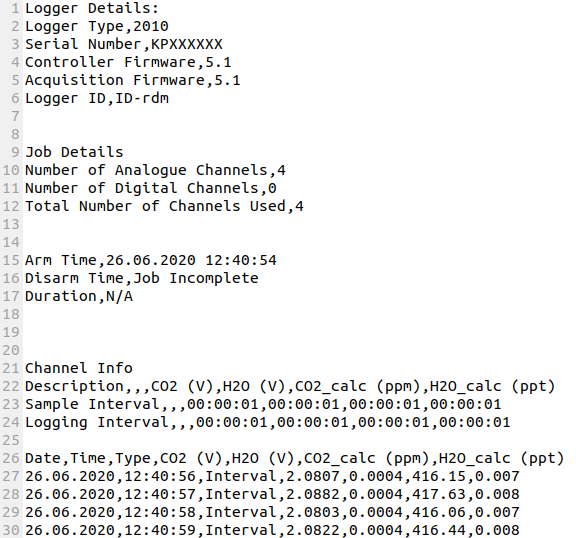
\includegraphics[width=0.7\linewidth,height=\textheight,keepaspectratio]{figures/squirrel_head.png}

}

\caption{\label{fig-header}Screenshot of the file
\texttt{26124054001.\#00} in a text editor. We can see that the 25th
first rows do not need to be imported, and that it is comma separated
with a dot as a decimal point.}

\end{figure}%

We will read the file with \texttt{read\_delim}, and then use
\texttt{rename} and \texttt{mutate} (from the \texttt{dplyr} package ;
Wickham \emph{et al.}, 2023) to transform the columns into what we want,
and \texttt{dmy\_hms} from the \texttt{lubridate} package (Grolemund and
Wickham, 2011) to get our datetime column in the right format:

\begin{Shaded}
\begin{Highlighting}[]
\FunctionTok{library}\NormalTok{(tidyverse)}
\CommentTok{\# readr, dplyr and lubridate are part of tidyverse}

\NormalTok{raw\_conc }\OtherTok{\textless{}{-}} \FunctionTok{read\_delim}\NormalTok{(}
  \StringTok{"ex\_data/26124054001.\#00"}\NormalTok{,}
  \AttributeTok{delim =} \StringTok{","}\NormalTok{, }\CommentTok{\# our file is comma separated}
  \AttributeTok{skip =} \DecValTok{25} \CommentTok{\# the first 25 rows are logger infos that we do not want to keep}
\NormalTok{)}
\end{Highlighting}
\end{Shaded}

\texttt{raw\_conc} structure:

\begin{verbatim}
#> spc_tbl_ [17 x 7] (S3: spec_tbl_df/tbl_df/tbl/data.frame)
#>  $ Date          : chr [1:17] "26.06.2020" "26.06.2020" "26.06.2020"..
#>  $ Time          : 'hms' num [1:17] 12:40:56 12:40:57 12:40:58 12:40..
#>  $ Type          : chr [1:17] "Interval" "Interval" "Interval" "Int"..
#>  $ CO2 (V)       : num [1:17] 2.08 2.09 2.08 2.08 2.06 ...
#>  $ H2O (V)       : num [1:17] 4e-04 4e-04 4e-04 4e-04 4e-04 4e-04 4e..
#>  $ CO2_calc (ppm): num [1:17] 416 418 416 416 412 ...
#>  $ H2O_calc (ppt): num [1:17] 0.007 0.008 0.007 0.008 0.008 0.007 0...
\end{verbatim}

Not too bad\ldots{} but we are not quite there yet:

\begin{itemize}
\tightlist
\item
  Some column names contain space
\item
  Some columns are not needed, removing them will make things easier
  later on: \texttt{Type} (nothing to do with the type of measurement,
  something from the logger), \texttt{CO2\ (V)}, \texttt{H2O\ (V)}
  (those two are the voltage input to the logger, not needed), and
  \texttt{H2O\_calc\ (ppt)} (that one was not calibrated for this
  campaign so better remove it to avoid confusion)
\item
  The \texttt{Date} and \texttt{Time} columns should be united in one
  and transformed in \texttt{yyyy-mm-dd\ hh:mm:ss} format
\end{itemize}

\begin{Shaded}
\begin{Highlighting}[]
\NormalTok{raw\_conc }\OtherTok{\textless{}{-}}\NormalTok{ raw\_conc }\SpecialCharTok{|\textgreater{}}
  \FunctionTok{rename}\NormalTok{(}
    \AttributeTok{co2\_conc =} \StringTok{"CO2\_calc (ppm)"}
\NormalTok{  ) }\SpecialCharTok{|\textgreater{}}
  \FunctionTok{mutate}\NormalTok{(}
    \AttributeTok{datetime =} \FunctionTok{paste0}\NormalTok{(Date, Time), }\CommentTok{\# we paste date and time together}
    \AttributeTok{datetime =} \FunctionTok{dmy\_hms}\NormalTok{(datetime) }\CommentTok{\# datetime instead of character}
\NormalTok{  ) }\SpecialCharTok{|\textgreater{}}
  \FunctionTok{select}\NormalTok{(datetime, co2\_conc)}
\end{Highlighting}
\end{Shaded}

\begin{verbatim}
#> tibble [17 x 2] (S3: tbl_df/tbl/data.frame)
#>  $ datetime: POSIXct[1:17], format: "2020-06-26 12:40:56" ...
#>  $ co2_conc: num [1:17] 416 418 416 416 412 ...
\end{verbatim}

\subsection{Importing multiple files}\label{importing-multiple-files}

Quite often a field season will result in several files. In this example
we will read all the files in ``ex\_data/'' that contain ``CO2'' in
their names.

\begin{Shaded}
\begin{Highlighting}[]
\FunctionTok{library}\NormalTok{(tidyverse)}

\NormalTok{raw\_conc }\OtherTok{\textless{}{-}} \FunctionTok{list.files}\NormalTok{( }\CommentTok{\# list the files}
  \StringTok{"ex\_data"}\NormalTok{, }\CommentTok{\# at location "ex\_data"}
  \AttributeTok{full.names =} \ConstantTok{TRUE}\NormalTok{,}
  \AttributeTok{pattern =} \StringTok{"*CO2*"} \CommentTok{\# that contains "CO2" in their name}
\NormalTok{) }\SpecialCharTok{|\textgreater{}}
  \FunctionTok{map\_dfr}\NormalTok{(}
\NormalTok{    read\_csv, }\CommentTok{\# we map read\_csv on all the files}
    \AttributeTok{na =} \FunctionTok{c}\NormalTok{(}\StringTok{"\#N/A"}\NormalTok{, }\StringTok{"Over"}\NormalTok{) }\CommentTok{\# "\#N/A" and Over should be treated as NA}
\NormalTok{  ) }\SpecialCharTok{|\textgreater{}}
  \FunctionTok{rename}\NormalTok{(}
    \AttributeTok{conc =} \StringTok{"CO2 (ppm)"}
\NormalTok{  ) }\SpecialCharTok{|\textgreater{}}
  \FunctionTok{mutate}\NormalTok{(}
    \AttributeTok{datetime =} \FunctionTok{dmy\_hms}\NormalTok{(}\StringTok{\textasciigrave{}}\AttributeTok{Date/Time}\StringTok{\textasciigrave{}}\NormalTok{)}
\NormalTok{  ) }\SpecialCharTok{|\textgreater{}}
  \FunctionTok{select}\NormalTok{(datetime, conc)}
\end{Highlighting}
\end{Shaded}

\subsection{The one file per flux approach}\label{sec-onefileflux}

\texttt{fluxible} can also be used with data that were recorded with one
file per flux and the file names as flux ID. In that case,
\texttt{flux\_match} can be skipped as we will directly import the data
with the flux IDs, and start and end of each flux measurements. In this
example we use the fluxible default column names to make it easier for
the rest of the data processing. The measurement lengths are based on
the start and end of the files, which might not be accurate depending on
the field routine. This can be adjusted with the arguments
\texttt{start\_cut}, \texttt{end\_cut} and \texttt{cut\_direction} in
\texttt{flux\_fitting}:

\begin{itemize}
\tightlist
\item
  \texttt{cut\_direction\ =\ "none"} (default) means the focus window is
  defined as \texttt{start\ +\ start\_cut} to \texttt{end\ -\ end\_cut}
\item
  \texttt{cut\_direction\ =\ "from\_start"} means the focus window is
  defined as \texttt{start\ +\ start\_cut} to
  \texttt{start\ +\ end\_cut}
\item
  \texttt{cut\_direction\ =\ "from\_end"} means the focus window is
  defined as \texttt{end\ -\ start\_cut} to \texttt{end\ -\ end\_cut}
\end{itemize}

\begin{Shaded}
\begin{Highlighting}[]
\FunctionTok{library}\NormalTok{(tidyverse)}

\NormalTok{raw\_conc }\OtherTok{\textless{}{-}} \FunctionTok{list.files}\NormalTok{( }\CommentTok{\#listing all the files}
  \StringTok{"ex\_data/field\_campaign"}\NormalTok{, }\CommentTok{\# at location "ex\_data/field\_campaign"}
  \AttributeTok{full.names =} \ConstantTok{TRUE}
\NormalTok{) }\SpecialCharTok{|\textgreater{}}
  \FunctionTok{map\_dfr}\NormalTok{( }\CommentTok{\# we map read\_tsv on all the files}
    \CommentTok{\# read\_tsv is the version of read\_delim for tab separated value files}
\NormalTok{    read\_tsv,}
    \AttributeTok{skip =} \DecValTok{3}\NormalTok{,}
    \CommentTok{\# creates a column with the filename, that we can use as flux ID}
    \AttributeTok{id =} \StringTok{"f\_fluxid"}
\NormalTok{  ) }\SpecialCharTok{|\textgreater{}}
  \FunctionTok{rename}\NormalTok{( }\CommentTok{\# a bit of renaming to make the columns more practical}
    \AttributeTok{co2\_conc =} \StringTok{"CO2 (umol/mol)"}\NormalTok{,}
    \AttributeTok{h2o\_conc =} \StringTok{"H2O (mmol/mol)"}\NormalTok{,}
    \AttributeTok{air\_temp =} \StringTok{"Temperature (C)"}\NormalTok{,}
    \AttributeTok{pressure =} \StringTok{"Pressure (kPa)"}
\NormalTok{  ) }\SpecialCharTok{|\textgreater{}}
  \FunctionTok{mutate}\NormalTok{(}
    \AttributeTok{.by =}\NormalTok{ f\_fluxid,}
    \AttributeTok{f\_datetime =} \FunctionTok{paste}\NormalTok{(Date, Time),}
    \CommentTok{\# we get rid of the milliseconds}
    \AttributeTok{f\_datetime =} \FunctionTok{as.POSIXct}\NormalTok{(f\_datetime, }\AttributeTok{format =} \StringTok{"\%Y{-}\%m{-}\%d \%H:\%M:\%OS"}\NormalTok{),}
    \AttributeTok{pressure =}\NormalTok{ pressure }\SpecialCharTok{/} \FloatTok{101.325}\NormalTok{, }\CommentTok{\# conversion from kPa to atm}
    \AttributeTok{f\_fluxid =} \FunctionTok{basename}\NormalTok{(f\_fluxid), }\CommentTok{\# removing folder names}
    \AttributeTok{f\_start =} \FunctionTok{min}\NormalTok{(f\_datetime), }\CommentTok{\# start is the smallest datetime of each flux}
    \AttributeTok{f\_end =} \FunctionTok{max}\NormalTok{(f\_datetime) }\CommentTok{\# end is the greatest datetime of each flux}
\NormalTok{  ) }\SpecialCharTok{|\textgreater{}}
  \FunctionTok{select}\NormalTok{(f\_datetime, co2\_conc, h2o\_conc, air\_temp,}
\NormalTok{         pressure, f\_fluxid, f\_start, f\_end)}
\end{Highlighting}
\end{Shaded}

\texttt{raw\_conc} structure:

\begin{verbatim}
#> tibble [18 x 8] (S3: tbl_df/tbl/data.frame)
#>  $ f_datetime: POSIXct[1:18], format: "2023-12-14 10:57:01" ...
#>  $ co2_conc  : num [1:18] 416 407 404 421 411 ...
#>  $ h2o_conc  : num [1:18] 22.7 22.5 23 22.6 22.8 ...
#>  $ air_temp  : num [1:18] 22.4 22.4 22.4 22.3 22.3 ...
#>  $ pressure  : num [1:18] 0.79 0.791 0.79 0.79 0.791 ...
#>  $ f_fluxid  : chr [1:18] "1_2000_east_1_day_a-2023-12-14T105700.tx"..
#>  $ f_start   : POSIXct[1:18], format: "2023-12-14 10:57:01" ...
#>  $ f_end     : POSIXct[1:18], format: "2023-12-14 10:57:06" ...
\end{verbatim}

\subsection{\texorpdfstring{The \texttt{licoread} R
package}{The licoread R package}}\label{sec-licoread}

The \texttt{licoread} R package (Gaudard, 2025) was developed to import
data files from LI-COR soil chamber systems in format 81x and 82z. It
follows the file structure logic from LI-COR, meaning that it should be
resilient to future updates and development or new instruments. It first
imports all the data as a nested dataframe (to make it lighter) with
\texttt{licoread}, and then produces a ``\texttt{fluxible}-friendly''
dataframe for the gas of focus with \texttt{licoread\_to\_fluxible}.

\subsubsection{Importing the data}\label{importing-the-data}

The data are imported with the \texttt{licoread} function. It needs the
location and the file type (if the folder is mixed, otherwise it is
determined automatically). The \texttt{sample\ =\ n} argument will
import a random sample of files of size n, which is convenient to test
code with a smaller sample of the data.

\begin{Shaded}
\begin{Highlighting}[]
\FunctionTok{library}\NormalTok{(licoread)}

\CommentTok{\# provide the location of your raw files to licoread}
\CommentTok{\# licoread reads subfolders as well}
\NormalTok{data }\OtherTok{\textless{}{-}} \FunctionTok{licoread}\NormalTok{(}
  \AttributeTok{location =} \StringTok{"ex\_data/82z"}\NormalTok{,}
  \CommentTok{\# sample = 10}
\NormalTok{  )}

\CommentTok{\# if your location containes more than one file type,}
\CommentTok{\# you will have to specify which files licoread should read}
\NormalTok{gas\_df\_82z }\OtherTok{\textless{}{-}} \FunctionTok{licoread}\NormalTok{(}\StringTok{"ex\_data/mixed\_files"}\NormalTok{, }\AttributeTok{file\_type =} \StringTok{"82z"}\NormalTok{)}
\end{Highlighting}
\end{Shaded}

\subsubsection{\texorpdfstring{Making a \texttt{fluxible}-friendly
dataframe}{Making a fluxible-friendly dataframe}}\label{making-a-fluxible-friendly-dataframe}

The \texttt{licoread\_to\_fluxible} function creates a dataframe with
\texttt{fluxible} default column names. Most of the time, LI-COR soil
chamber system will measure several gases simultaneously. The
\texttt{focus\_gas} argument tells which gas should be present in this
dataframe. See Appendix \ref{sec-twogases} for the processing of several
gases measured simultaneously.

\begin{Shaded}
\begin{Highlighting}[]
\NormalTok{gas\_df\_81x }\OtherTok{\textless{}{-}} \FunctionTok{licoread}\NormalTok{(}\StringTok{"ex\_data/81x"}\NormalTok{)}

\NormalTok{co2\_df }\OtherTok{\textless{}{-}} \FunctionTok{licoread\_to\_fluxible}\NormalTok{(}
  \AttributeTok{df =}\NormalTok{ gas\_df\_81x,}
  \AttributeTok{focus\_gas =} \StringTok{"CO2"}\NormalTok{,}
  \AttributeTok{datetime\_col =} \StringTok{"Date"}
\NormalTok{)}
\end{Highlighting}
\end{Shaded}

With the 82z file type, the name of measured gases is less intuitive
(because it includes the name of the instruments). The
\texttt{list\_gases()} function lists all the gases present in the
dataset.

\begin{Shaded}
\begin{Highlighting}[]
\FunctionTok{list\_gases}\NormalTok{(gas\_df\_82z)}
\CommentTok{\#\textgreater{} File type is 82z.}
\CommentTok{\#\textgreater{} [1] "LI{-}7810\_CH4\_DRY" "LI{-}7810\_CO2\_DRY" "LI{-}7820\_N2O\_DRY" "LI{-}7825\_CO2"}
\end{Highlighting}
\end{Shaded}

\begin{Shaded}
\begin{Highlighting}[]
\NormalTok{ch4\_dry }\OtherTok{\textless{}{-}} \FunctionTok{licoread\_to\_fluxible}\NormalTok{(}
  \AttributeTok{df =}\NormalTok{ gas\_df\_82z,}
  \AttributeTok{focus\_gas =} \StringTok{"LI{-}7810\_CH4\_DRY"}\NormalTok{,}
  \AttributeTok{datetime\_col =} \FunctionTok{c}\NormalTok{(}\StringTok{"LI{-}8250\_DATE"}\NormalTok{, }\StringTok{"LI{-}8250\_TIME"}\NormalTok{)}
\NormalTok{)}
\end{Highlighting}
\end{Shaded}

\section{\texorpdfstring{Using \texttt{fluxible} with two gases measured
simultaneously}{Using fluxible with two gases measured simultaneously}}\label{sec-twogases}

In this example we will process the \texttt{raw\_twogases} dataset which
contains both CO\textsubscript{2} and CH\textsubscript{4} concentrations
measured simultaneously. The aim is a single dataset of fluxes in which
the CH\textsubscript{4} fluxes were also discarded when the
CO\textsubscript{2} fluxes were discarded.

The concept is that we will treat the dataset twice, once for each gas,
and then join them again in the end. Because \texttt{f\_fluxid} is
produced in chronological order based on start datetime in
\texttt{field\_record}, the fluxes measured at the same time have the
same \texttt{f\_fluxid}.

First we use \texttt{flux\_match} to slice the raw concentration data
and attribute a unique ID to each measurement.

\begin{Shaded}
\begin{Highlighting}[]
\FunctionTok{library}\NormalTok{(fluxible)}
\FunctionTok{library}\NormalTok{(dplyr)}

\NormalTok{conc\_twogases }\OtherTok{\textless{}{-}} \FunctionTok{flux\_match}\NormalTok{(}
  \AttributeTok{raw\_conc =}\NormalTok{ raw\_twogases,}
  \AttributeTok{field\_record =}\NormalTok{ twogases\_record,}
  \AttributeTok{f\_datetime =}\NormalTok{ datetime,}
  \AttributeTok{start\_col =}\NormalTok{ start,}
  \AttributeTok{measurement\_length =} \DecValTok{180}\NormalTok{,}
  \AttributeTok{time\_diff =} \DecValTok{0}
\NormalTok{)}
\end{Highlighting}
\end{Shaded}

Then we fit a model to the raw data for each gas:

\begin{Shaded}
\begin{Highlighting}[]
\NormalTok{slopes\_twogases\_co2 }\OtherTok{\textless{}{-}} \FunctionTok{flux\_fitting}\NormalTok{(}
  \AttributeTok{conc\_df =}\NormalTok{ conc\_twogases,}
  \AttributeTok{f\_conc =}\NormalTok{ co2\_conc,}
  \AttributeTok{f\_datetime =}\NormalTok{ datetime,}
  \AttributeTok{fit\_type =} \StringTok{"exp\_zhao18"}\NormalTok{,}
  \AttributeTok{start\_cut =} \DecValTok{10}
\NormalTok{)}

\NormalTok{slopes\_twogases\_ch4 }\OtherTok{\textless{}{-}} \FunctionTok{flux\_fitting}\NormalTok{(}
  \AttributeTok{conc\_df =}\NormalTok{ conc\_twogases,}
  \AttributeTok{f\_conc =}\NormalTok{ ch4\_conc,}
  \AttributeTok{f\_datetime =}\NormalTok{ datetime,}
  \AttributeTok{fit\_type =} \StringTok{"exp\_zhao18"}\NormalTok{,}
  \AttributeTok{start\_cut =} \DecValTok{10}
\NormalTok{)}
\end{Highlighting}
\end{Shaded}

Same with the quality, we do it once for each gas:

\begin{Shaded}
\begin{Highlighting}[]
\NormalTok{flag\_twogases\_co2 }\OtherTok{\textless{}{-}} \FunctionTok{flux\_quality}\NormalTok{(}
  \AttributeTok{slopes\_df =}\NormalTok{ slopes\_twogases\_co2,}
  \AttributeTok{f\_conc =}\NormalTok{ co2\_conc,}
  \AttributeTok{force\_discard =} \StringTok{"8"} \CommentTok{\# peak at the start that is probably an error}
\NormalTok{)}
\CommentTok{\#\textgreater{} }
\CommentTok{\#\textgreater{}  Total number of measurements: 12}
\CommentTok{\#\textgreater{} }
\CommentTok{\#\textgreater{}  ok   11      92 \%}
\CommentTok{\#\textgreater{}  force\_discard    1   8 \%}
\CommentTok{\#\textgreater{}  discard      0   0 \%}
\CommentTok{\#\textgreater{}  zero     0   0 \%}
\CommentTok{\#\textgreater{}  start\_error      0   0 \%}
\CommentTok{\#\textgreater{}  no\_data      0   0 \%}
\CommentTok{\#\textgreater{}  force\_ok     0   0 \%}
\CommentTok{\#\textgreater{}  force\_zero   0   0 \%}
\CommentTok{\#\textgreater{}  force\_lm     0   0 \%}
\CommentTok{\#\textgreater{}  no\_slope     0   0 \%}

\NormalTok{flag\_twogases\_ch4 }\OtherTok{\textless{}{-}} \FunctionTok{flux\_quality}\NormalTok{(}
  \AttributeTok{slopes\_df =}\NormalTok{ slopes\_twogases\_ch4,}
  \AttributeTok{f\_conc =}\NormalTok{ ch4\_conc,}
  \AttributeTok{ambient\_conc =} \DecValTok{2000} \CommentTok{\# default is for CO2}
\NormalTok{)}
\CommentTok{\#\textgreater{} }
\CommentTok{\#\textgreater{}  Total number of measurements: 12}
\CommentTok{\#\textgreater{} }
\CommentTok{\#\textgreater{}  ok   9   75 \%}
\CommentTok{\#\textgreater{}  zero     3   25 \%}
\CommentTok{\#\textgreater{}  discard      0   0 \%}
\CommentTok{\#\textgreater{}  force\_discard    0   0 \%}
\CommentTok{\#\textgreater{}  start\_error      0   0 \%}
\CommentTok{\#\textgreater{}  no\_data      0   0 \%}
\CommentTok{\#\textgreater{}  force\_ok     0   0 \%}
\CommentTok{\#\textgreater{}  force\_zero   0   0 \%}
\CommentTok{\#\textgreater{}  force\_lm     0   0 \%}
\CommentTok{\#\textgreater{}  no\_slope     0   0 \%}
\end{Highlighting}
\end{Shaded}

We check the fits with \texttt{flux\_plot}
(Figure~\ref{fig-co2-twogases} and Figure~\ref{fig-ch4-twogases}).

\begin{Shaded}
\begin{Highlighting}[]
\NormalTok{flag\_twogases\_co2 }\SpecialCharTok{|\textgreater{}}
  \FunctionTok{flux\_plot}\NormalTok{(}
    \AttributeTok{f\_conc =}\NormalTok{ co2\_conc,}
    \AttributeTok{f\_datetime =}\NormalTok{ datetime,}
    \AttributeTok{f\_ylim\_upper =} \DecValTok{500}\NormalTok{,}
    \AttributeTok{f\_ylim\_lower =} \DecValTok{425}\NormalTok{,}
    \AttributeTok{y\_text\_position =} \DecValTok{460}
\NormalTok{  )}
\end{Highlighting}
\end{Shaded}

\begin{figure}[H]

\centering{

\pandocbounded{\includegraphics[keepaspectratio]{fluxible_appendix_files/figure-pdf/fig-co2-twogases-1.pdf}}

}

\caption{\label{fig-co2-twogases}CO\textsubscript{2} measurements with
quality flags.}

\end{figure}%

\begin{Shaded}
\begin{Highlighting}[]
\NormalTok{flag\_twogases\_ch4 }\SpecialCharTok{|\textgreater{}}
  \FunctionTok{flux\_plot}\NormalTok{(}
    \AttributeTok{f\_conc =}\NormalTok{ ch4\_conc,}
    \AttributeTok{f\_datetime =}\NormalTok{ datetime,}
    \AttributeTok{f\_ylim\_upper =} \DecValTok{2000}\NormalTok{,}
    \AttributeTok{f\_ylim\_lower =} \DecValTok{1995}\NormalTok{,}
    \AttributeTok{y\_text\_position =} \DecValTok{1997}
\NormalTok{  )}
\end{Highlighting}
\end{Shaded}

\begin{figure}[H]

\centering{

\pandocbounded{\includegraphics[keepaspectratio]{fluxible_appendix_files/figure-pdf/fig-ch4-twogases-1.pdf}}

}

\caption{\label{fig-ch4-twogases}CH\textsubscript{4} measurements with
quality flags.}

\end{figure}%

After calculating the fluxes, we need to rename the \texttt{f\_flux}
column to avoid confusion when joining the datasets:

\begin{Shaded}
\begin{Highlighting}[]
\NormalTok{fluxes\_twogases\_co2 }\OtherTok{\textless{}{-}} \FunctionTok{flux\_calc}\NormalTok{(}
  \AttributeTok{slopes\_df =}\NormalTok{ flag\_twogases\_co2,}
  \AttributeTok{slope\_col =}\NormalTok{ f\_slope\_corr,}
  \AttributeTok{f\_datetime =}\NormalTok{ datetime,}
  \AttributeTok{temp\_air\_col =}\NormalTok{ temp\_air,}
  \AttributeTok{conc\_unit =} \StringTok{"ppm"}\NormalTok{,}
  \AttributeTok{flux\_unit =} \StringTok{"mmol/m2/h"}\NormalTok{,}
  \AttributeTok{setup\_volume =} \FloatTok{6.31}\NormalTok{,}
  \AttributeTok{atm\_pressure =} \DecValTok{1}\NormalTok{,}
  \AttributeTok{plot\_area =} \FloatTok{0.31}\NormalTok{,}
  \CommentTok{\# we want to use the quality flags of CO2 to eventally discard CH4 fluxes}
  \AttributeTok{cols\_keep =} \StringTok{"f\_quality\_flag"}
\NormalTok{) }\SpecialCharTok{|\textgreater{}}
\FunctionTok{rename}\NormalTok{( }\CommentTok{\# to avoid any confusion, we rename the flux column}
  \AttributeTok{flux\_co2 =} \StringTok{"f\_flux"}
\NormalTok{) }\SpecialCharTok{|\textgreater{}} \CommentTok{\# and we remove the slope one}
\FunctionTok{select}\NormalTok{(}\SpecialCharTok{{-}}\NormalTok{f\_slope\_corr)}

\NormalTok{fluxes\_twogases\_ch4 }\OtherTok{\textless{}{-}} \FunctionTok{flux\_calc}\NormalTok{(}
  \AttributeTok{slopes\_df =}\NormalTok{ flag\_twogases\_ch4,}
  \AttributeTok{slope\_col =}\NormalTok{ f\_slope\_corr,}
  \AttributeTok{f\_datetime =}\NormalTok{ datetime,}
  \AttributeTok{temp\_air\_col =}\NormalTok{ temp\_air,}
  \AttributeTok{conc\_unit =} \StringTok{"ppb"}\NormalTok{, }\CommentTok{\# ch4 is measured in ppb}
  \AttributeTok{flux\_unit =} \StringTok{"umol/m2/h"}\NormalTok{, }\CommentTok{\# we want a flux in umol/m2/h}
  \AttributeTok{setup\_volume =} \FloatTok{6.31}\NormalTok{,}
  \AttributeTok{atm\_pressure =} \DecValTok{1}\NormalTok{,}
  \AttributeTok{plot\_area =} \FloatTok{0.31}
\NormalTok{) }\SpecialCharTok{|\textgreater{}}
\FunctionTok{rename}\NormalTok{( }\CommentTok{\# to avoid any confusion, we rename the flux column}
  \AttributeTok{flux\_ch4 =} \StringTok{"f\_flux"}
\NormalTok{) }\SpecialCharTok{|\textgreater{}} \CommentTok{\# and we remove the slope one}
\FunctionTok{select}\NormalTok{(}\SpecialCharTok{{-}}\NormalTok{f\_slope\_corr)}
\end{Highlighting}
\end{Shaded}

Then we can join the datasets. If the final dataset ends up being
longer, it probably means that some values in columns that should be
equal (\texttt{f\_temp\_air\_ave} for example) are in fact not equal,
which leads to additional rows when joining the dataframes.

\begin{Shaded}
\begin{Highlighting}[]
\NormalTok{fluxes\_twogases }\OtherTok{\textless{}{-}} \FunctionTok{left\_join}\NormalTok{(}
\NormalTok{  fluxes\_twogases\_co2,}
\NormalTok{  fluxes\_twogases\_ch4,}
  \AttributeTok{by =} \FunctionTok{c}\NormalTok{(}
  \CommentTok{\# if that does not work, then it means that we did}
  \CommentTok{\# something different for one of the gases}
    \StringTok{"f\_fluxid"}\NormalTok{,}
    \StringTok{"f\_temp\_air\_ave"}\NormalTok{,}
    \StringTok{"datetime"}\NormalTok{,}
    \StringTok{"f\_model"}
\NormalTok{    )}
\NormalTok{) }\SpecialCharTok{|\textgreater{}}
\FunctionTok{mutate}\NormalTok{( }\CommentTok{\# we discard the CH4 fluxes based on CO2 fluxes quality flags}
  \AttributeTok{flux\_ch4 =} \FunctionTok{case\_when}\NormalTok{(}
\NormalTok{    f\_quality\_flag }\SpecialCharTok{\%in\%} \FunctionTok{c}\NormalTok{(}\StringTok{"discard"}\NormalTok{, }\StringTok{"force\_discard"}\NormalTok{) }\SpecialCharTok{\textasciitilde{}} \ConstantTok{NA}\NormalTok{,}
    \AttributeTok{.default =}\NormalTok{ flux\_ch4}
\NormalTok{  )}
\NormalTok{)}
\end{Highlighting}
\end{Shaded}

Structure of \texttt{fluxes\_twogases}:

\begin{verbatim}
#> tibble [12 x 7] (S3: tbl_df/tbl/data.frame)
#>  $ f_quality_flag: chr [1:12] "ok" "ok" "ok" "ok" ...
#>  $ f_fluxid      : Factor w/ 12 levels "1","2","3","4",..: 1 2 3 4 5..
#>  $ f_temp_air_ave: num [1:12] 13.4 16.5 17.1 14.4 15 ...
#>  $ datetime      : POSIXct[1:12], format: "2024-06-18 10:04:37" ...
#>  $ flux_co2      : num [1:12] 0.08292 0.38505 0.43518 0.00108 0.0637..
#>  $ f_model       : chr [1:12] "exp_zhao18" "exp_zhao18" "exp_zhao18"..
#>  $ flux_ch4      : num [1:12] -0.04873 0.01165 0 -0.00649 0 ...
\end{verbatim}

In this example we calculated the fluxes for two gases measured
simultaneously by repeating the process for each gas, and in the end we
joined them and applied a rule that discarded the fluxes of one gas
based on the quality flags of the other. It is of course totally
possible to apply other rules, or to just keep the fluxes as provided by
\texttt{fluxible}.

\section{\texorpdfstring{Brief overview of the \texttt{exp\_zhao18}
exponential
model}{Brief overview of the exp\_zhao18 exponential model}}\label{sec-theory}

The exponential model \texttt{exp\_zhao18} is described in Zhao \emph{et
al.} (2018). They, however, do not describe how to automatically fit
this model to real data. They recommend using the \texttt{optim}
function (R Core Team, 2024) on the root mean square error (RMSE) for
each flux. This approach requires starting points which are specific to
each measurement. As \texttt{optim} is quite sensitive to the choice of
starting points, and that this equation, with four fitting parameters
(\(C_m\), \(a\), \(b\), and \(t_0\)), has a large number of minima, it
is critical to approximate the starting points as close as possible to
the real values. When working flux after flux, it would not be too
difficult to manually estimate them. \texttt{fluxible}, however, aims to
automate this step. This section describes the steps that are happening
in the \texttt{flux\_fitting\_zhao18} function, which is a non-exported
function called by \texttt{flux\_fitting} when using the
\texttt{exp\_zhao18} model.

The gas concentration as a function of time is defined as follows:
\begin{equation}\phantomsection\label{eq-zhao}{
C(t) = C_m + a(t - t_0) + (C_0 - C_m) \exp( - b(t - t_0))
}\end{equation}

This model can fit both linear and exponential fluxes. When \(a = 0\),
the term \((t - t_0)\) is cancelled and the model becomes the HM model:

\[
C(t) = C_m + (C_0 - C_m)\exp(-b(t-t_0))
\]

And when \(b=0\), then \(\exp(-b(t-t_0)) = 1\):

\[
C(t) = C_0 + a (t - t_0) + (C-z - C_m)
\]

After simplification, what is left is a linear model:

\[
C(t)=C_0 + a(t - t_0)
\]

The slope to calculate the gas flux is the derivative of
Equation~\ref{eq-zhao} at \(t_0\):

\[
C'(t_0)=0 + a + (-b) (C_0 - C_m) \exp( - b(t_0 - t_0))
\]

Which after simplification becomes:

\begin{equation}\phantomsection\label{eq-slope}{
C'(t_0)=a + b (C_m - C_0)
}\end{equation}

\subsection{Description of the terms}\label{description-of-the-terms}

The term \(a(t - t_0)\) is here to correct the flux in case of a peak or
a dip resulting from a leak (ER) or condensation (NEE) or temperature
increase (both). Therefore, the first part of the flux, before a peak or
a dip, can be described without this term:

\begin{equation}\phantomsection\label{eq-licor}{
C(t)=C_m+(C_0 - C_m)\exp(-b(t-t_0))
}\end{equation}

The term \((C_0 - C_m)\exp(-b(t-t_0))\) describes the exponential
relationship of the gas concentration over time and \(C_m\) is the
``maximum mixing ratio when equilibrium is established between the soil
and the air in the chamber''. \(C_0\) is defined as the intercept of the
linear fit of a short period at the beginning of the flux (called
\(C_{z\_window}\)). In a perfectly linear flux \(C_0=C(0)\). For an
ideal undisturbed measurement, Equation~\ref{eq-licor} would be
sufficient.

\subsection{Estimation of fitting
parameters}\label{estimation-of-fitting-parameters}

The fitting parameters of the exponential model are determined using
\texttt{optim()} on the root mean square error (RMSE) for each flux:

\begin{equation}\phantomsection\label{eq-rmse}{
\text{RMSE}=\sqrt{\frac{1}{N}\sum_{i = 1}^N(P_i-O_i)^2}
}\end{equation} Where \(P_i\) are the predicated values and \(O_i\) the
observed.

The raw data are fitted to a series of simpler models whose parameters
are used as starting points for \texttt{optim}. In the following steps,
the suffix \(\_est\) (for ``estimated'') indicates the starting point of
the corresponding parameter.

\(C_m\) is estimated (\(C_{m\_est}\)) as either the lowest gas
concentration value in case of an overall decreasing gas concentration
in the chamber, or the highest in case of an increasing concentration.

\(t_0\) is defined as \(C(t_0) = C_0\). \(t_0\) can only be positive as
it is not defined before the measurement starts. \(t_{z\_est}\) is
estimated as the time when observed gas concentration is the closest to
\(C_0\). To avoid undesirable effects of outliers, a rolling mean (15
seconds interval by default) is applied to gas concentration data. Only
the first half of the measurement is used to estimate \(t_{z\_est}\) to
avoid using gas concentration data situated after a peak or a dip.

\(b_{est}\) can be calculated using \(C_{m\_est}\) and \(C_0\) and an
arbitrary time \(t_b=t_0-b_{window}\) (10 seconds as default parameter)
and an estimation of \(C(t_b)\) (called \(C_b\)) by looking at the
observed gas value at \(t_b\):

\[
b_{est}=\log(|\frac{C_b-C_{m\_est}}{C_0-C_{m\_est}}|) \times \frac{1}{b_{window}}
\]

Once the starting points for C\textsubscript{m}, t\textsubscript{z} and
b are estimated and C\textsubscript{z} provided, \(a(t - t_0)\) can be
re-introduced in Equation~\ref{eq-licor} to correct the part of the flux
following a potential peak (or dip). Following the same idea as for
\(b_{est}\), \(a_{est}\) can be calculated using the other estimates and
a time window at the end of the flux (the last 10 seconds by default).

\[
a_{est}=\frac{(C_a - C_{m\_est} - (C_0 - C_{m\_est}) * \exp(-b_{est} * (t_a - t_{z\_est})))}{(t_a - t_{z\_est})}
\] \(t_a\) being the length of the flux minus \(a_{window}\) and \(C_a\)
the observed gas concentration at \(t_a\).

Finally, the \texttt{optim()} function is run on Equation~\ref{eq-rmse}
with predicted values from Equation~\ref{eq-zhao} and starting points
provided as described above.

\blandscape

\section{Quality flags}\label{sec-qualityflags}

\small

\begin{longtable}[]{@{}
  >{\raggedright\arraybackslash}p{(\linewidth - 6\tabcolsep) * \real{0.3200}}
  >{\raggedright\arraybackslash}p{(\linewidth - 6\tabcolsep) * \real{0.3500}}
  >{\raggedright\arraybackslash}p{(\linewidth - 6\tabcolsep) * \real{0.1300}}
  >{\raggedright\arraybackslash}p{(\linewidth - 6\tabcolsep) * \real{0.2000}}@{}}
\caption{\normalsize Quality assessment with \texttt{flux\_quality} when
using a linear model. Criteria are applied in descending
order.}\label{tbl-flagslm}\tabularnewline
\toprule\noalign{}
\begin{minipage}[b]{\linewidth}\raggedright
Criteria
\end{minipage} & \begin{minipage}[b]{\linewidth}\raggedright
Meaning
\end{minipage} & \begin{minipage}[b]{\linewidth}\raggedright
Quality flag
\end{minipage} & \begin{minipage}[b]{\linewidth}\raggedright
Recommended slope
\end{minipage} \\
\midrule\noalign{}
\endfirsthead
\toprule\noalign{}
\begin{minipage}[b]{\linewidth}\raggedright
Criteria
\end{minipage} & \begin{minipage}[b]{\linewidth}\raggedright
Meaning
\end{minipage} & \begin{minipage}[b]{\linewidth}\raggedright
Quality flag
\end{minipage} & \begin{minipage}[b]{\linewidth}\raggedright
Recommended slope
\end{minipage} \\
\midrule\noalign{}
\endhead
\bottomrule\noalign{}
\endlastfoot
\texttt{f\_fluxid} in \texttt{force\_discard} & User has reasons to
discard this flux. & \texttt{force\_discard} & \texttt{NA} \\
\texttt{f\_fluxid} in \texttt{force\_ok} & User has reasons to keep this
flux. & \texttt{force\_ok} & As estimated by \texttt{flux\_fitting} \\
\texttt{f\_fluxid} in \texttt{force\_zero} & User has reasons to replace
this flux with 0. & \texttt{force\_zero} & 0 \\
\texttt{f\_ratio} = 0 (no data) & Measurement has no data. &
\texttt{no\_data} & \texttt{NA} \\
\texttt{f\_ratio} \textless{} \texttt{ratio\_threshold} & Measurement is
missing too many data. & \texttt{discard} & \texttt{NA} \\
\(|\text{avg first 3 datapoints} -\) \texttt{ambient\_conc}\(| >\)
\texttt{error} & Measurement is starting outside of realistic range of
ambient concentration. & \texttt{start\_error} & \texttt{NA} \\
\texttt{is.na(f\_slope)\ =\ TRUE} & Model could not be fit to gas
concentration data. & \texttt{no\_slope} & \texttt{NA} \\
R\^{}2 \(\geq\) \texttt{rsquared\_threshold} & The fit is good. &
\texttt{ok} & As estimated by \texttt{flux\_fitting} \\
R\^{}2 \textless{} \texttt{rsquared\_threshold} \& p-value \(\geq\)
\texttt{pvalue\_threshold} & The fit is bad and the concentration is not
changing over time. & \texttt{zero} & 0 \\
R\^{}2 \textless{} \texttt{rsquared\_threshold} \& p-value \textless{}
\texttt{pvalue\_threshold} \& \texttt{f\_slope} \(\leq\)
\texttt{f\_min\_slope} & The fit is bad and the slope is below the
minimal detectable slope. & \texttt{zero} & 0 \\
R\^{}2 \textless{} \texttt{rsquared\_threshold} \& p-value \textless{}
\texttt{pvalue\_threshold} \& \texttt{f\_slope} \textgreater{}
\texttt{f\_min\_slope} & The fit is bad. & \texttt{discard} &
\texttt{NA} \\
\end{longtable}

\newpage
\small

\begin{longtable}[]{@{}
  >{\raggedright\arraybackslash}p{(\linewidth - 6\tabcolsep) * \real{0.3200}}
  >{\raggedright\arraybackslash}p{(\linewidth - 6\tabcolsep) * \real{0.3500}}
  >{\raggedright\arraybackslash}p{(\linewidth - 6\tabcolsep) * \real{0.1300}}
  >{\raggedright\arraybackslash}p{(\linewidth - 6\tabcolsep) * \real{0.2000}}@{}}
\caption{\normalsize Quality assessment with \texttt{flux\_quality} when
using a quadratic model. Criteria are applied in descending
order.}\label{tbl-flagsqua}\tabularnewline
\toprule\noalign{}
\begin{minipage}[b]{\linewidth}\raggedright
Criteria
\end{minipage} & \begin{minipage}[b]{\linewidth}\raggedright
Meaning
\end{minipage} & \begin{minipage}[b]{\linewidth}\raggedright
Quality flag
\end{minipage} & \begin{minipage}[b]{\linewidth}\raggedright
Recommended slope
\end{minipage} \\
\midrule\noalign{}
\endfirsthead
\toprule\noalign{}
\begin{minipage}[b]{\linewidth}\raggedright
Criteria
\end{minipage} & \begin{minipage}[b]{\linewidth}\raggedright
Meaning
\end{minipage} & \begin{minipage}[b]{\linewidth}\raggedright
Quality flag
\end{minipage} & \begin{minipage}[b]{\linewidth}\raggedright
Recommended slope
\end{minipage} \\
\midrule\noalign{}
\endhead
\bottomrule\noalign{}
\endlastfoot
\texttt{f\_fluxid} in \texttt{force\_discard} & User has reasons to
discard this flux. & \texttt{force\_discard} & \texttt{NA} \\
\texttt{f\_fluxid} in \texttt{force\_ok} & User has reasons to keep this
flux. & \texttt{force\_ok} & As estimated by \texttt{flux\_fitting} \\
\texttt{f\_fluxid} in \texttt{force\_zero} & User has reasons to replace
this flux with 0. & \texttt{force\_zero} & 0 \\
\texttt{f\_fluxid} in \texttt{force\_lm} & User has reasons to use the
linear slope for this flux. & \texttt{force\_lm} & As estimated by
\texttt{flux\_fitting} (linear model) \\
\texttt{f\_ratio} = 0 (no data) & Measurement has no data. &
\texttt{no\_data} & \texttt{NA} \\
\texttt{f\_ratio} \textless{} \texttt{ratio\_threshold} & Measurement is
missing too many data. & \texttt{discard} & \texttt{NA} \\
\(|\text{avg first 3 datapoints} -\) \texttt{ambient\_conc}\(| >\)
\texttt{error} & Measurement is starting outside of realistic range of
ambient concentration. & \texttt{start\_error} & \texttt{NA} \\
\texttt{is.na(f\_slope)\ =\ TRUE} & Model could not be fit to gas
concentration data. & \texttt{no\_slope} & \texttt{NA} \\
\texttt{f\_gfactor} \textgreater{} \texttt{gfactor\_threshold}

\& \texttt{f\_slope\_lm} \textgreater{} \texttt{f\_min\_slope} & Slope
is too different from linear slope and above the minimal detectable
slope. & \texttt{discard} & \texttt{NA} \\
\texttt{f\_gfactor} \textgreater{} \texttt{gfactor\_threshold}

\& \texttt{f\_slope\_lm} \(\leq\) \texttt{f\_min\_slope} & Slope is too
different from linear slope and is below the minimal detectable slope. &
\texttt{zero} & 0 \\
\(R^2 \geq\) \texttt{rsquared\_threshold} & The fit is good. &
\texttt{ok} & As estimated by \texttt{flux\_fitting} \\
\(R^2\) \textless{} \texttt{rsquared\_threshold} \& p-value \(\geq\)
\texttt{pvalue\_threshold} & The fit is bad and the concentration is not
changing over time. & \texttt{zero} & 0 \\
\(R^2\) \textless{} \texttt{rsquared\_threshold} \& p-value \textless{}
\texttt{pvalue\_threshold} \& \texttt{f\_slope} \(\leq\)
\texttt{f\_min\_slope} & The fit is bad and the slope is below the
minimal detectable slope. & \texttt{zero} & 0 \\
\(R^2\) \textless{} \texttt{rsquared\_threshold} \& p-value \textless{}
\texttt{pvalue\_threshold} \& \texttt{f\_slope} \textgreater{}
\texttt{f\_min\_slope} & The fit is bad. & \texttt{discard} &
\texttt{NA} \\
\end{longtable}

\newpage
\small

\begin{longtable}[]{@{}
  >{\raggedright\arraybackslash}p{(\linewidth - 6\tabcolsep) * \real{0.3200}}
  >{\raggedright\arraybackslash}p{(\linewidth - 6\tabcolsep) * \real{0.3500}}
  >{\raggedright\arraybackslash}p{(\linewidth - 6\tabcolsep) * \real{0.1300}}
  >{\raggedright\arraybackslash}p{(\linewidth - 6\tabcolsep) * \real{0.2000}}@{}}
\caption{\normalsize Quality assessment with \texttt{flux\_quality} when
using an exponential model. Criteria are applied in descending
order.}\label{tbl-flagsexp}\tabularnewline
\toprule\noalign{}
\begin{minipage}[b]{\linewidth}\raggedright
Criteria
\end{minipage} & \begin{minipage}[b]{\linewidth}\raggedright
Meaning
\end{minipage} & \begin{minipage}[b]{\linewidth}\raggedright
Quality flag
\end{minipage} & \begin{minipage}[b]{\linewidth}\raggedright
Recommended slope
\end{minipage} \\
\midrule\noalign{}
\endfirsthead
\toprule\noalign{}
\begin{minipage}[b]{\linewidth}\raggedright
Criteria
\end{minipage} & \begin{minipage}[b]{\linewidth}\raggedright
Meaning
\end{minipage} & \begin{minipage}[b]{\linewidth}\raggedright
Quality flag
\end{minipage} & \begin{minipage}[b]{\linewidth}\raggedright
Recommended slope
\end{minipage} \\
\midrule\noalign{}
\endhead
\bottomrule\noalign{}
\endlastfoot
\texttt{f\_fluxid} in \texttt{force\_discard} & User has reasons to
discard this flux. & \texttt{force\_discard} & \texttt{NA} \\
\texttt{f\_fluxid} in \texttt{force\_ok} & User has reasons to keep this
flux. & \texttt{force\_ok} & As estimated by \texttt{flux\_fitting} \\
\texttt{f\_fluxid} in \texttt{force\_zero} & User has reasons to replace
this flux with 0. & \texttt{force\_zero} & 0 \\
\texttt{f\_fluxid} in \texttt{force\_lm} & User has reasons to use the
linear slope for this flux. & \texttt{force\_lm} & As estimated by
\texttt{flux\_fitting} (linear model) \\
\texttt{f\_ratio} = 0 (no data) & Measurement has no data. &
\texttt{no\_data} & \texttt{NA} \\
\texttt{f\_ratio} \textless{} \texttt{ratio\_threshold} & Measurement is
missing too many data. & \texttt{discard} & \texttt{NA} \\
\(|\text{avg first 3 datapoints} -\) \texttt{ambient\_conc}\(| >\)
\texttt{error} & Measurement is starting outside of realistic range of
ambient concentration. & \texttt{start\_error} & \texttt{NA} \\
\texttt{is.na(f\_slope)\ =\ TRUE} & Model could not be fit to gas
concentration data. & \texttt{no\_slope} & \texttt{NA} \\
\texttt{f\_gfactor} \textgreater{} \texttt{gfactor\_threshold}

\& \texttt{f\_slope\_lm} \textgreater{} \texttt{f\_min\_slope} & Slope
is too different from linear slope and above the minimal detectable
slope. & \texttt{discard} & \texttt{NA} \\
\texttt{f\_gfactor} \textgreater{} \texttt{gfactor\_threshold}

\& \texttt{f\_slope\_lm} \(\leq\) \texttt{f\_min\_slope} & Slope is too
different from linear slope and below the minimal detectable slope. &
\texttt{zero} & 0 \\
(\(|b| \geq\) \texttt{b\_threshold} or

\(\text{RMSE} >\) \texttt{rmse\_threshold})

\& \(|\)\texttt{f\_cor\_coef}\(| \geq\) \texttt{cor\_threshold}

\& \texttt{f\_slope\_lm} \textgreater{} \texttt{f\_min\_slope} & The fit
is bad \& the concentration is changing over time \& the slope is
detectable. & \texttt{discard} & \texttt{NA} \\
(\(|b| \geq\) \texttt{b\_threshold} or

\(\text{RMSE} >\) \texttt{rmse\_threshold})

\& \(|\)\texttt{f\_cor\_coef}\(| \geq\) \texttt{cor\_threshold}

\& \texttt{f\_slope\_lm} \(\leq\) \texttt{f\_min\_slope} & The fit is
bad \& the slope is not detectable. & \texttt{zero} & 0 \\
(\(|b| \geq\) \texttt{b\_threshold} or

\(\text{RMSE} >\) \texttt{rmse\_threshold})

\& \(|\)\texttt{f\_cor\_coef}\(| <\) \texttt{cor\_threshold} & The fit
is bad \& the concentration is not changing over time. & \texttt{zero} &
0 \\
\(\text{RMSE} \leq\) \texttt{rmse\_threshold} & The fit is good. &
\texttt{ok} & As estimated by \texttt{flux\_fitting} \\
\end{longtable}

\normalsize

\elandscape

\newpage

\section{List of functions}\label{sec-listfct}

\begin{longtable}[]{@{}
  >{\raggedright\arraybackslash}p{(\linewidth - 2\tabcolsep) * \real{0.2500}}
  >{\raggedright\arraybackslash}p{(\linewidth - 2\tabcolsep) * \real{0.7500}}@{}}
\caption{List of available functions in \texttt{fluxible}
1.3.0.}\label{tbl-allfcts}\tabularnewline
\toprule\noalign{}
\begin{minipage}[b]{\linewidth}\raggedright
Function
\end{minipage} & \begin{minipage}[b]{\linewidth}\raggedright
Brief description
\end{minipage} \\
\midrule\noalign{}
\endfirsthead
\toprule\noalign{}
\begin{minipage}[b]{\linewidth}\raggedright
Function
\end{minipage} & \begin{minipage}[b]{\linewidth}\raggedright
Brief description
\end{minipage} \\
\midrule\noalign{}
\endhead
\bottomrule\noalign{}
\endlastfoot
\texttt{flux\_match} & Matches continuous gas concentration data with
metadata \\
\texttt{flux\_drygas} & Wet air correction \\
\texttt{flux\_fitting} & Fits a model to the flux measurements \\
\texttt{flux\_quality} & Assesses the quality of the fits \\
\texttt{flux\_flag\_count} & Provides the counts of quality flags in a
dataframe (for reporting) \\
\texttt{flux\_plot} & Plots the flux measurements with their fits and
quality flags \\
\texttt{flux\_calc} & Calculates fluxes \\
\texttt{flux\_diff} & Calculates the difference between paired fluxes,
for gross primary production (GPP) and transpiration \\
\texttt{flux\_gpp} & Same as \texttt{flux\_diff} but specific to GPP
(superseded, \texttt{flux\_diff} offers more flexibility) \\
\texttt{flux\_lrc} & Standardises CO\textsubscript{2} fluxes at fixed
PAR values \\
\texttt{flux\_units} & Unit conversion coefficient for fluxes (used
inside \texttt{flux\_calc}) \\
\texttt{stupeflux} & Wrapper including \texttt{flux\_match},
\texttt{flux\_fitting}, \texttt{flux\_quality} and \texttt{flux\_calc}
(for performance testing) \\
\end{longtable}

\section*{References}\label{references}
\addcontentsline{toc}{section}{References}

\phantomsection\label{refs}
\begin{CSLReferences}{1}{0}
\bibitem[\citeproctext]{ref-gaudardLicoreadReadsRaw2025}
Gaudard, J. (2025), \emph{Licoread: {Reads} Raw Files from Li-{COR} Gas
Analyzers}, Manual, available
at:\url{https://doi.org/10.32614/CRAN.package.licoread}.

\bibitem[\citeproctext]{ref-lubridate2011}
Grolemund, G. and Wickham, H. (2011), {``Dates and times made easy with
{lubridate}''}, \emph{Journal of Statistical Software}, Vol. 40 No. 3,
pp. 1--25.

\bibitem[\citeproctext]{ref-hutchinsonImprovedSoilCover1981}
Hutchinson, G.L. and Mosier, A.R. (1981),
{``\href{https://doi.org/10.2136/sssaj1981.03615995004500020017x}{Improved
{Soil Cover Method} for {Field Measurement} of {Nitrous Oxide
Fluxes}}''}, \emph{Soil Science Society of America Journal}, Vol. 45 No.
2, pp. 311--316.

\bibitem[\citeproctext]{ref-rcoreteamLanguageEnvironmentStatistical2024}
R Core Team. (2024), \emph{R: A Language and Environment for Statistical
Computing}, Manual, R Foundation for Statistical Computing, Vienna,
Austria.

\bibitem[\citeproctext]{ref-vandvikPlantTraitsAssociated2025}
Vandvik, V., Halbritter, A.H., Macias-Fauria, M., Maitner, B.S.,
Michaletz, S.T., Telford, R.J., Bison, N., \emph{et al.} (2025),
{``\href{https://doi.org/10.1038/s41597-025-05509-4}{Plant traits and
associated ecological data from global change experiments and climate
gradients in {Norway}}''}, \emph{Scientific Data}, Nature Publishing
Group, Vol. 12 No. 1, p. 1477.

\bibitem[\citeproctext]{ref-tidyverse2019}
Wickham, H., Averick, M., Bryan, J., Chang, W., McGowan, L.D., François,
R., Grolemund, G., \emph{et al.} (2019),
{``\href{https://doi.org/10.21105/joss.01686}{Welcome to the
{tidyverse}}''}, \emph{Journal of Open Source Software}, Vol. 4 No. 43,
p. 1686.

\bibitem[\citeproctext]{ref-dplyr2023}
Wickham, H., François, R., Henry, L., Müller, K. and Vaughan, D. (2023),
\emph{Dplyr: A Grammar of Data Manipulation}, Manual, available
at:\url{https://doi.org/10.32614/CRAN.package.dplyr}.

\bibitem[\citeproctext]{ref-readr2024}
Wickham, H., Hester, J. and Bryan, J. (2024), \emph{Readr: {Read}
Rectangular Text Data}, Manual, available
at:\url{https://doi.org/10.32614/CRAN.package.readr}.

\bibitem[\citeproctext]{ref-zhaoCalculationDaytimeCO22018}
Zhao, P., Hammerle, A., Zeeman, M. and Wohlfahrt, G. (2018),
{``\href{https://doi.org/10.1016/j.agrformet.2018.08.022}{On the
calculation of daytime {CO2} fluxes measured by automated closed
transparent chambers}''}, \emph{Agricultural and Forest Meteorology},
Vol. 263, pp. 267--275.

\end{CSLReferences}




\end{document}
